\documentclass[journal,twoside,web]{ieeecolor2}
\usepackage{generic}
\usepackage{cite}
\usepackage{amsmath,amssymb,amsfonts}
\usepackage{algorithmic}
\usepackage{graphicx}
\usepackage{textcomp}
\def\BibTeX{{\rm B\kern-.05em{\sc i\kern-.025em b}\kern-.08em
    T\kern-.1667em\lower.7ex\hbox{E}\kern-.125emX}}
\markboth{\journalname, VOL. XX, NO. XX, XXXX 2023}
{Author \MakeLowercase{\textit{et al.}}: Preparation of Papers for IEEE TRANSACTIONS and JOURNALS (December 2023)}
\begin{document}
\title{Preparation of Paper (Stage 1): Counting pages and fitting the figures}
\author{First A. Author, \IEEEmembership{Fellow, IEEE}, Second B. Author, and Third C. Author, Jr., \IEEEmembership{Member, IEEE}
\thanks{This paragraph of the first footnote will contain the date on 
which you submitted your paper for review. It will also contain support 
information, including sponsor and financial support acknowledgment. For 
example, ``This work was supported in part by the U.S. Department of 
Commerce under Grant BS123456.'' }
\thanks{The next few paragraphs should contain 
the authors' current affiliations, including current address and e-mail. For 
example, F. A. Author is with the National Institute of Standards and 
Technology, Boulder, CO 80305 USA (e-mail: author@boulder.nist.gov). }
\thanks{S. B. Author, Jr., was with Rice University, Houston, TX 77005 USA. He is 
now with the Department of Physics, Colorado State University, Fort Collins, 
CO 80523 USA (e-mail: author@lamar.colostate.edu).}
\thanks{T. C. Author is with 
the Electrical Engineering Department, University of Colorado, Boulder, CO 
80309 USA, on leave from the National Research Institute for Metals, 
Tsukuba, Japan (e-mail: author@nrim.go.jp).}}

\maketitle

\begin{abstract}
These instructions give you guidelines for preparing papers for 
IEEE Transactions and Journals. Use this document as a template if you are 
using \LaTeX. Otherwise, use this document as an 
instruction set. The electronic file of your paper will be formatted further 
at IEEE. Paper titles should be written in uppercase and lowercase letters, 
not all uppercase. Avoid writing long formulas with subscripts in the title; 
short formulas that identify the elements are fine (e.g., "Nd--Fe--B"). Do 
not write ``(Invited)'' in the title. Full names of authors are preferred in 
the author field, but are not required. Put a space between authors' 
initials. The abstract must be a concise yet comprehensive reflection of 
what is in your article. In particular, the abstract must be self-contained, 
without abbreviations, footnotes, or references. It should be a microcosm of 
the full article. The abstract must be between 150--250 words. Be sure that 
you adhere to these limits; otherwise, you will need to edit your abstract 
accordingly. The abstract must be written as one paragraph, and should not 
contain displayed mathematical equations or tabular material. The abstract 
should include three or four different keywords or phrases, as this will 
help readers to find it. It is important to avoid over-repetition of such 
phrases as this can result in a page being rejected by search engines. 
Ensure that your abstract reads well and is grammatically correct.
\end{abstract}

\begin{IEEEkeywords}
Acoustic distortion,
auditory system,
biharmonic spline interpolation,
distortion measurement,
distortion product otoacoustic emissions,
delaunay triangulation,
ear,
shape,
shape measurement
\end{IEEEkeywords}

\section{Introduction}
\label{sec:introduction}
\subsection{DPOAE, DPOAE Input-output functions and DPOAE level maps for assessment of the cochlear amplifier}
Distortion-product otoacoustic emissions (DPOAE) are sound waves generated in the nonlinear, active cochlea through the intermodulation of two-tone stimulation, characterized by the stimulus frequencies $f_1$ and $f_2$ and their stimulus levels $L_1$ and $L_2$. DPOAE can be measured in the ear canal. In humans, the most pronounced DPOAEs are observed at the 3rd order product frequency $f_{DP} = 2f_1 - f_2$. In clinical practice, DPOAEs are used as a diagnostic tool to evaluate the function of the cochlear amplifier (Davis, 1983), typically with fixed frequency ratio set to approx. $f_2 / f_1 = 1.2$ to maximize response amplitude (Gaskill and Brown, 1990). Several approaches have been made to establish an optimal standard paradigm for DPOAE measurements to assess the state of the so-called cochlear amplifier. These approaches differ primarily in the amount of dimensions of the parameter space.

The method most commonly used in clinical settings, known as a DP-Gram, measures DPOAE at a single combination of stimulus levels (often $L_2, L_1 = 55, 65 dB$ SPL) for each frequency (Abdala, 2001), and thus represents a one-dimensional scan. The diagnostic information sought, i.e. the state of the cochlear amplifier, has a highly nonlinear and quite variable relation to the DPOAE amplitudes (Gorga et al. 1996, Bhatt et al. 2023). Therefore, a normative range is defined within which the amplitudes should fall if the cochlear amplifier is functioning normally. This approach leads to a dichotomous diagnostic result, indicating whether or not the cochlear amplifier is healthy (Probst et al., 1991, Lonsbury-Martin and Martin, 2003 in Current opinion in otolaryngology head and neck surgery)).

A more advanced approach, DPOAE input-output (I/O) functions, uses multiple level combinations where the stimulus-tone levels are linearly related (Kummer et al., 1998). In this method, the DPOAE pressure responses are plotted as a function of the level of the second primary. DPOAE input-output (I/O) functions enhance diagnostic sensitivity for detecting cochlear-amplifier-related hearing loss (Gaskill and Brown, 1990; Stover, 1996). When extrapolated from semi-logarithmically scaled I/O functions, this approach provides an almost linear relationship between DPOAE threshold and pure-tone hearing threshold (Boege \& Janssen, 2002; Gorga et al., 2003). Importantly, this method allows the use of inclusion criteria that are independent of signal-to-noise ratio (SNR) thereby improving diagnostic reliability (Zelle et al. 2017) .

Finally, DPOAE can be sampled at a range of independent level combinations creating a three-dimensional representation in the $(L_2, L_1)$-plane, thus adding a third dimension to the data recorded per given frequency $f_2$.

This approach, which we refer here to as DPOAE level map (LM) was initially introduced by Whitehead (1995) and Kummer (2000). DPOAE LMs of limited density or extent can also be derived from investigations on DPOAE amplitude dependence on one stimulus level alone, e.g. [Brown \& Gaskill, 1990, Neely 2005]. All mentioned reports used prescribed level combinations, which we refer to as static level maps (SLMs), to investigate DPOAE generation characteristics, primarily focusing on identifying group-optimal stimulus paths in the $(L_2, L_1)$-plane that lead to maximum DPOAE levels. Zelle et al., 2015 reported on DPOAE LMs based on pulsed DPOAE using the onset decomposition (OD) method that eliminates artefacts caused by the interference of the two competing source contributions: the nonlinear-distortion component and the coherent reflection component [Zelle, Thiericke 2015]. The OD method samples the rising onset of the DPOAE signal in the time domain before the low-latency reflection component begins to interfere. As a result, “smooth” DPOAE LMs with a clear maximum allow a more precise representation of the state of the cochlear amplifier and thus increase the diagnostic value (Zelle et al., 2015, Zelle et al., 2020).
 

\subsection{DPOAE level dependence}
Experimental evidence from multiple studies (Cooper 1997, Whitehead 1995, Kummer 2000, Zelle 2015, Zelle2020) indicates that DPOAE LMs in mammalians, including humans, exhibit a common characteristic, particularly at low-to-moderate stimulus levels ($L_2<50 dB$ SPL). This characteristic manifests as a distinct ridge (see Fig. 1A) representing the maximum DPOAE amplitudes stimulated by the minimal stimulus pressure, i.e. at optimal combinations of $L_1$ and $L_2$. The ridge’s projection onto the $(L_2, L_1)$-plane yields the level combinations that can be considered individually optimal for each ear (Zelle 2020).

The structure of DPOAE LMs can be roughly approximated by a 5-parameter model ( ref patent Ernst \& Zelle 2020 ). This model implies that the ridge is a line in a defined $(L_2, L_1, p_{DP})$-space with parabolic cross section when DPOAEs are scaled as level ($L_{DP}=20 log_{10} (p_{DP}/20 \mu Pa$), with $p_{DP}$ being the sound pressure of the DPOAE). The line itself is described by four parameters: ($a, b, s$ and $L_{2,EDPT}$), where $s$ is a slope in $\mathbb{R}^3$-space, $a$ - the slope of the optimum path in the $(L_2, L_1)$-plane, $b$ is its $L_1$-intercept, and $L_{2,EDPT}$ is the intercept of the ridge line with the $(L_2, L_1)$-plane. The cross-section perpendicular to the ridge line as well as the $(L_2, L_1)$-plane is provided by a 5th parameter $c$, which expands the line to a model surface with a parabolic law dependent on the level of the DPOAE, $L_{DP}$ (Zelle et al. 2020).

In experimental practice, however, the ridge of a DPOAE LM is not always a straight line, the shape of the surface can deviate characteristically from the 5-parameter model, and the ridge’s position may vary significantly between individuals. Ridge position and slope are affected by pathological but also non-pathological middle-ear transduction changes, such as minor static middle-ear pressure changes (Zitat janssen ). Together with off-ridge points characterizing the general shape of the map, the estimated ridge representing the DPOAE I/O function may provide the clinically most important information about the DPOAE LM, as it may not only allow the estimation of the hearing threshold but also represents compressive nonlinearity and allows predictions about the functional state of the cochlear amplifier independent of threshold (Abdala et al., 2021). It is, though, understood, that the regular shape of DPOAE LMs can be compromised by several factors, e.g. spontaneous otoacoustic emissions (SOAE), SNR, or time variance during measurement.


\subsection{Aim of a new method to derive DPOAE level maps}
To efficiently acquire the individual shape of a DPOAE LM, it is crucial to employ an adaptive measurement algorithm. Traditional methods, which rely on predefined or static level combinations, may sometimes fail to capture the unique characteristics of each subject’s DPOAE response, leading to suboptimal diagnostic accuracy and collection of redundant data. 

In this article we introduce a method for adaptive DPOAE level-map acquisition that is capable of autonomous exploration of a level map based on the existence of DPOAE responses and their amplitudes, and that can be tailored to different research or clinical needs. 

Another aim is to assess all forms of LMs not limited to only a priori assumptions about the shape of the map such as those inherent in the 5-parameter model presented in [Zelle 2020]. Specifically for the derivation of a subject-specific optimal path that might not necessarily be linear in the  $(L_2, L_1)$-plane. With respect to clinical needs, the adaptive scanning algorithms investigated here might serve in future to collect DPOAE data containing the complete three-dimensional information in a most time-efficient manner.

The DPOAE LM approach requires the measurement of more DPOAE than a DPOAE I/O function. In turn, it offers two significant advantages: 1) Measuring a DPOAE LM reveals the individually optimal path. Once known, a measurement of an I/O function along this path or its derivation from the DPOAE LM provides a more accurate representation of DPOAE growth properties compared to measurements of DPOAE I/O functions along a group-optimal path (s. Fig. 0 and Zelle et al., 2020).  Fig. 0 shows an extreme case of two DPOAE LM from normal-hearing subjects which would lead to misleading results when measured with DPOAE I/O functions along a group-optimal path. 2) Characteristic shifts of the DPOAE LM and accompanying reductions of the amplitudes of their ridge are known to be produced by conductive hearing loss, i.e. reductions of middle-ear transmission, and can therefore potentially be used for differential diagnostics of middle- and inner-ear impairments and lead to higher specificity for the diagnosis of the state of the cochlear amplifier (Janssen et al., 2005, Kummer, 2006, Turcanu, 2009, Steffen, 2017). 

The here introduced adaptive measurement algorithm not only enhances the precision of the map but also significantly optimizes the time required for data acquisition, making it a more efficient and reliable method for clinical diagnostics.

\section{Methods}
\subsection{Measurement system and calibration}
OAE measurements were performed bilaterally using an ER-10C DPOAE probe system (Etymotic Research, Elk Grove Village, IL, USA) connected to a 16-bit analog output card and a 24-bit signal acquisition card (NI PCI 6733 and NI PCI 4472, National Instruments, Austin, TX, USA) situated in a commercially available PC. The sampling frequency was 102.4 kHz. Stimulus generation and data acquisition were controlled by a custom-built toolbox implemented in LabVIEW (version 14.0, National Instruments, Austin, TX, USA). The sound pressure of the ER-10C speakers was ascertained by in-ear SPL calibration, which was repeated every 600 s. Both the output of the speakers and the recorded microphone signal were corrected for the transfer functions of an artificial ear simulator (B\&K type 4157, Brüel \& Kjær, Nærum, Denmark) and of the ER-10C microphone to yield DPOAEs, which are considered to correspond to recordings close to the tympanic membrane. Further details of the calibration routine are given elsewhere ( Zelle et al., 2015a ). Signal post-processing and data analysis were done in MATLAB (version 9.12, MathWorks, Natick, MA, USA).

\subsection{DPOAE acquisition – Static level maps}
SLMs are DPOAE LMs that are recorded using predefined $(L_2, L_1)$-stimulus level combinations. The aim is to capture the expected position of the DPOAE LM with an appropriate region around the ridge, based on the population mean parameters of the group optimum path for different frequencies. The stimulus level combinations for SLM were adapted from (Zelle 2020) and slightly modified especially at high stimulus levels. The resulting grid had lateral symmetry about the expected group-mean optimum path ($L_2'$-axis, cf. Fig. 1B), fixed distances ($10 dB$ along the $L_2'$-axis, and $6 dB$ along the $L_1'$-axis). It comprises six cross sections of the expected level map with 3, 4, 5, 3, 3, 3 points per scan along the L1'-axis (see Fig. 4, red pattern). The position of the grid is defined by $(L_{2,MIN} , L_{1,MIN})$, s. Fig. 4, for values,  s. Sec. V, Table 1), which were based on the experience from previous experiments (Bader et al., 2021) to optimize data yield in normal-hearing subjects.

\subsection{DPOAE acquisition – Adaptive level maps}
Adaptive LMs (ALMs) are defined as DPOAE LMs that are procedurally generated to increase the efficiency of DPOAE acquisition. In other words, after measuring a prescribed starting point, the algorithm selects the next stimulus level combinations depending on the configuration of assessed and modelled data. An initial level combination (i.e. $p_1^1$ on Fig. 1, panel B) is chosen in a frequency-dependent manner with $L_{2,START} = 55 dB$ for $f_2 < 4 kHz$, 60 dB for $f_2 < 8 kHz$, and $65 dB$ for larger $f_2$, while $L_1$ is linearly bound with $L_2$ according to Zelle 2020 (see Table I, Sec. V ).  In principle, all adaptive methods described here can be utilized stand-alone or in conjunction, depending on the particular clinical or research task. We subdivide the adaptive methods into two groups.

\begin{figure*}
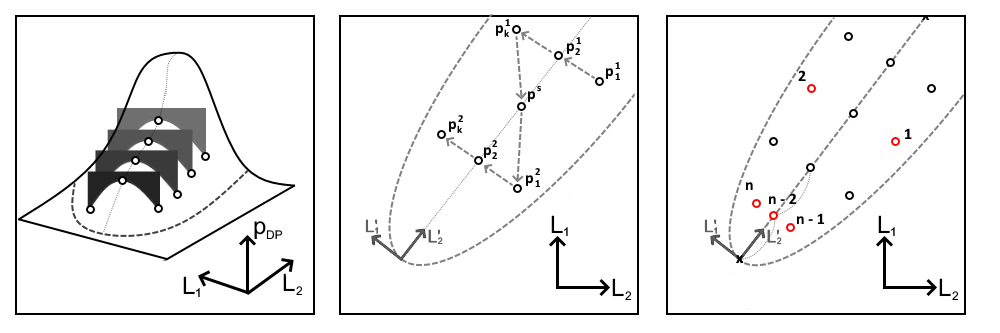
\includegraphics[width=\textwidth]{Fig_ALM_ModelBased} %,height=4cm
\caption{Model-based algorithms to identify the ridge of DPOAE LMs: A: Model surface of an ideal DPOAE LM, described via perpendicular scans, illustrating the expected structure of a typical DPOAE LM. B: Ridge estimator method. To minimize the number of points per measurement, this method employs two ridge scans ($p^1_i$ and $p^2_i$) and one intermediate point $p^s$. Ideally, it samples seven points to estimate all major characteristics of the DPOAE LM. C: Ridge follower method. This method strongly relies on the estimated DPOAE LM surface and is used to enhance the resolution of points along the ridge. It requires a minimum of three points per scan (the ridge point and one point on either side) and provides a prescribed overall amount of scans perpendicular to the ridge.}
\label{fig_AMB}
\end{figure*}

The first group of ALM acquisition methods relies on the expected shape of a DPOAE level map, i.e., it uses a priori knowledge as discussed in Section I.C, and shown in Fig. 1A. Two methods belong to the a priori group: the so-called ridge estimator and ridge follower. To simplify the description of the ALM methods, we refer to a $(L_2’, L_1’)$-plane which is rotated such that the projection of the ridge onto the $(L_2, L_1)$-plane aligns with the $L_2'$ axis (s. Fig. 1B).  The angle of the rotation corresponds to the group mean slope-parameter "a" (s. Sec. I.B, and Zelle 2020).
The ridge estimator ( ref to patent ) is utilized to verify the presence of the presumed DPOAE LM and to roughly estimate model surface properties. The algorithm is comprised of three steps – two ridge scans and one intermediate point (see Fig. 1A for ridge and Fig. 1B for illustration of the ridge estimator algorithm):
\begin{algorithmic}[1]
\STATE An initial ridge scan $p_k^1$ samples the presumed ridge along $L_1'$ starting from an initial level combination $p_1^1$ and aims to detect its maximum to prove the existence of a ridge. Every single ridge scan might take up to $k$ DPOAE amplitudes or points (here: $k=4$), limited by a pre-defined region of interest (ROI). The ROI might be tailored to specific tasks, but typically will contain an upper limit for $L_2$ and $L_1$ to avoid acoustic overstimulation and/or technical distortions (here: $95 dB$ SPL). Sampling during a ridge scan has two modes: 1) if there are no accepted DPOAE amplitudes or points, the $L_1'$ increment is set to $10 dB$, 2) if the acquired DPOAE adhere to the predefined acceptance criteria (based on SNR, s. Sec. II.D), the $L_1'$ increment is set to $6 dB$. If the detected DPOAE amplitude $p_{DP}$ decreases after two successful measurements, the $L_1'$ increment is switched to be negative. Once three DPOAE have been accepted, the maximum is determined by solving a quadratic equation to their levels. If four attempts fail to determine a ridge, an additional scan is deployed on half distance between the existing scan and upper ROI boundaries.
\STATE Once a maximum within a ridge scan is detected, an intermediate point $p^s$ is sampled to estimate individually the slope of the ridge. This point is positioned based on the assumed frequency dependence of the slope s of the group mean optimal path, a (Zelle 2020, their Table I) and on the typical background noise levels – such that it is expected to fall on half distance between the first scan and the location where the prescribed minimum SNR for an accepted DPOAE would be obtained. In this study, $SNR_{MIN}$ was set to $10 dB$.
\STATE After the slope of the DPOAE LM ridge is individually computed, a starting point for the 2nd low-level scan perpendicular to the ridge is set at a $L_2'$ where a $SNR = SNR_{MIN} + 12 dB$ is expected. This value was chosen empirically as a compromise between the goals to obtain valid DPOAEs at low stimulus-levels and to avoid measuring neighbouring off-ridge points without achieving the required SNR. After measuring an initial point, the second scan $p_k^2$ is performed in the same manner as $p_k^1$ (see step 1).
\end{algorithmic} 

The second acquisition method of the \textit{a priori} group is the "ridge follower". This method involves two recurrent steps (see Fig. 1C) aimed at enhancing the resolution of the DPOAE data along the ridge:
\begin{algorithmic}[1]
\STATE For any existing singular point on the ridge (e.g., $p^s$ in Fig. 1B), two satellite points are assigned on either side of the ridge.
\STATE If no singular points are left, a new point (s. Fig. 1C: $n – 2$) is positioned on the ridge. The longest empty interval, either between the ROI boundaries and the nearest point or between existing points along the ridge, is identified, and the new point is placed by bisecting the interval.
\end{algorithmic} 

A second group of "data-based" acquisition methods was implemented, relying solely on the already existing points based on Delaunay triangulation (Lee, D.T., Schachter, B.J., 1980) referred to as"polygonal search method" (PSM). The PSM and terms used in the following are borrowed from graph theory. It comprises two cases – the general and the expansive case.

\begin{figure*}
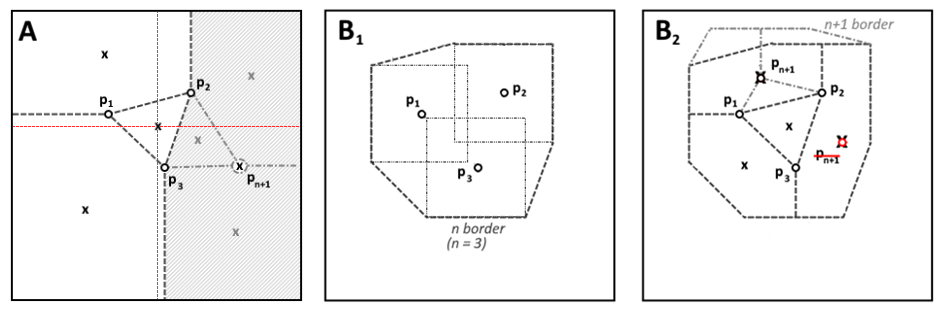
\includegraphics[width=\textwidth]{Fig_ALM_DataBased} %,height=4cm
\caption{Data-based algorithm to identify DPOAE LM without a priori assumptions on its shape. A situation may arise where certain points have been measured, but the model surface cannot be accessed. In such cases, an algorithm is used that systematically searches for data points in the $(L_2, L_1)$ level depending on the SNR. A: A general case of Polygonal Search Method (PSM) splits the ROI into smaller polygons and takes the centre of mass ($p_{n+1}$, marked as cross) of the biggest polygon (marked with gray) to be measured next. B: An expansion case of PSM, which is a stricter version of general case. It bases its prediction only on “accepted” points in two steps: firstly it assesses the boundaries (n border) based on given vicinity area of accepted point (it has a square shape), secondly it runs a general case of PSM within new boundaries to estimate the next point.}
\label{fig_ADB}
\end{figure*}

In the general case of the PSM (see Fig. 2A), any existing points with all kind of DPOAE amplitudes within the boundaries of the ROI are considered. The data-based algorithm consists of the following steps:
\begin{algorithmic}[1]
\STATE All points which have already been measured (continuous-line circles in Fig. 2A, $p_{1...3}$), are processed with a Delaunay triangulation function (matlab function \textit{delaunayTriangulation(P)}) that generates triangle polygons, based on those and defined via vertices coordinates list and triangular faces  connectivity list (Lee, D.T., Schachter, B.J., 1980; see their Appendix B).
\STATE To construct polygons adjacent to boundaries of the ROI, the vertices of the alpha shape of all acquired points, i.e. the circumference of the set of triangles, are connected to the boundaries of the ROI according to the minimum-distance principle (vertical and horizontal lines in Fig. 2A). To prevent edge clustering, the $(L_2, L_1)$-plane is divided into four sections by two orthogonal lines (see red dashed lines in Fig. 2A) intersecting at the centre of mass of the alpha shape. Points can only be connected to a boundary located in the same section.
\STATE Once all connections between the points and the boundaries are established, the updated connectivity list contains all non-overlapping polygons within the ROI. The largest polygon (see gray polygon in Fig. 2A) is selected and its centre of mass is chosen as the next measurement point.
\end{algorithmic} 

If PSM is applied without prior data, the subdivision of the $(L_2, L_1)$-plane (step 2) begins in a pre-described initial point and creates four different polygons. Following this step, the method continues with the aforementioned steps.

In the expansion case of the PSM, only points with accepted DPOAE amplitudes are taken into account and the ROI is redefined based on those points in every step. For each accepted point, neighbouring points defining a group are identified by their distances with $\delta L_2 \le 10 dB$, $\delta L_1 \le 15 dB$. Around these points, a square-shaped region of pre-defined size is built (here: $20 \times 20 dB$), and their common circumference is yielding a polygon, which describes the new ROI (s. Fig. 2B$_1$, dashed line). Following these rules, more than one ROI can appear. The final step is to employ the general case for all groups simultaneously, meaning that the largest polygon identified in any group generates the next point (s. Fig. 2C). The expansion case has the advantage to constrain the ROI to an area where the probability might be deemed high to lead to accepted DPOAE.

\subsection{Study design and subjects}

The pilot study, validating the adaptive algorithm for DPOAE LM acquisition, included three normal-hearing subjects (age: 27, 31 and 37 years old). All three subjects were classified as normal-hearing as all pure-tone thresholds were better than 20 dB hearing level (dB HL) for frequencies between 1 and 8 kHz.

DPOAE LMs were recorded bilaterally at 14 frequencies ranging from 1 to 14 kHz ($f_2 = 1, 1.5, 2, 3, 4, 5, 6, 8, 9, 10, 11, 12, 13, 14 kHz$), yielding 84 independent data sets. The stimulus and recording sequence are based on a time-interlaced multi-frequency acquisition technique (Zelle, 2014).  21 level combinations per frequency were chosen, each of which averaged over 44 ensembles comprising four blocks with appropriate phase shifts to apply the PTPV technique. Within a block of length of 0.18 seconds, 7 frequencies are presented in a time-interlaced manner; the whole measurement including intermittent calibrations took approximately 25 minutes. For each measured DPOAE amplitude, we performed sorted averaging, estimated the noise floor and, if SNR exceeds 10 dB, the corresponding point was considered accepted. The noise floor was estimated as the root-mean-square of the difference between two subsets of the underlying segments from the DPOAE recording in a 50-ms time interval centred on the DPOAE response. The subsets were created by averaging two sets of interlaced PTPV ensembles, each of which contained four consecutive segments with suitable phase variations to cancel the stimulus pulses. 

\begin{figure}[ht]
\centerline{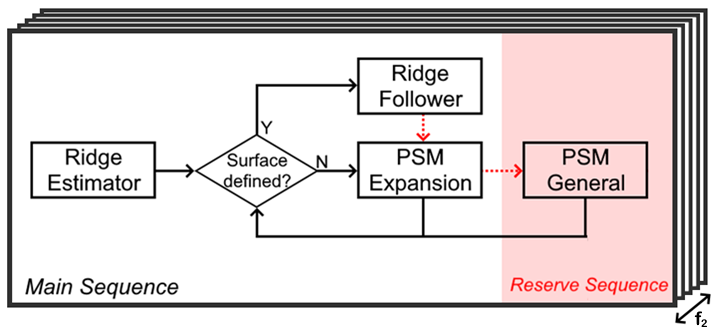
\includegraphics[width=\columnwidth]{Fig_Sequence.png}}
\caption{Adaptive acquisition workflow: Black arrows – regular sequence, red arrows – exception sequence (if measurement at prescribed point is not possible for any reason).}
\label{fig_SQS}
\end{figure}

The sequence of measurements used in this study is depicted in Fig. 3. After assessment of  pure-tone thresholds using a Békésy tracking method (for details: Bader et al., 2021) , DPOAE are acquired with ALM followed by SLM in a subsequent visit after 1-2 months. During ALM acquisition (see Section II.C), the sequence of a priori and data-based acquisition methods is followed independently for each frequency stimulated within a block. The sequence is organized such, that after completion of the ridge estimator, every two measurements, the model is fitted to all hitherto assessed DPOAE amplitudes. The 5-parameter model is accepted if the following criteria are met: $r^2 > 0.8, \sigma \le 10$, where $r$ is the correlation coefficient between DPOAE amplitudes and the 5-parameter model fitted to them, and $\sigma $ is standard error of the model parameter $L_{2, EDPT}$ (Zelle et al., 2020; see Section I B). If these criteria are satisfied, the ridge follower algorithm complements the level map, if not, the PSM expansion method is initiated. 

The study was approved by the Ethics Committee of the University of Tübingen and   was conducted in accordance with the Declaration of Helsinki for human experiments.

\subsection{Post-processing and analysis}

\subsubsection{Connectivity-based analysis}
To compare and analyse SLM and ALM without relying on the surface shape produced by the DPOAE, we use quantities that are present in each measurement: number of all acquired points ($N_{all}$), number of points with accepted DPOAE amplitudes ($N_{acc}$), and the area of the alpha shape ($S$) of $N_{acc}$ (s. Fig. 4). Additionally, for post-processing here we restrict the connectivity list such, that it does not have triangles with edges larger than 18 dB, to minimize the influence from extrapolation artefacts, which might take place in next subsection.

\begin{figure}[ht]
\centerline{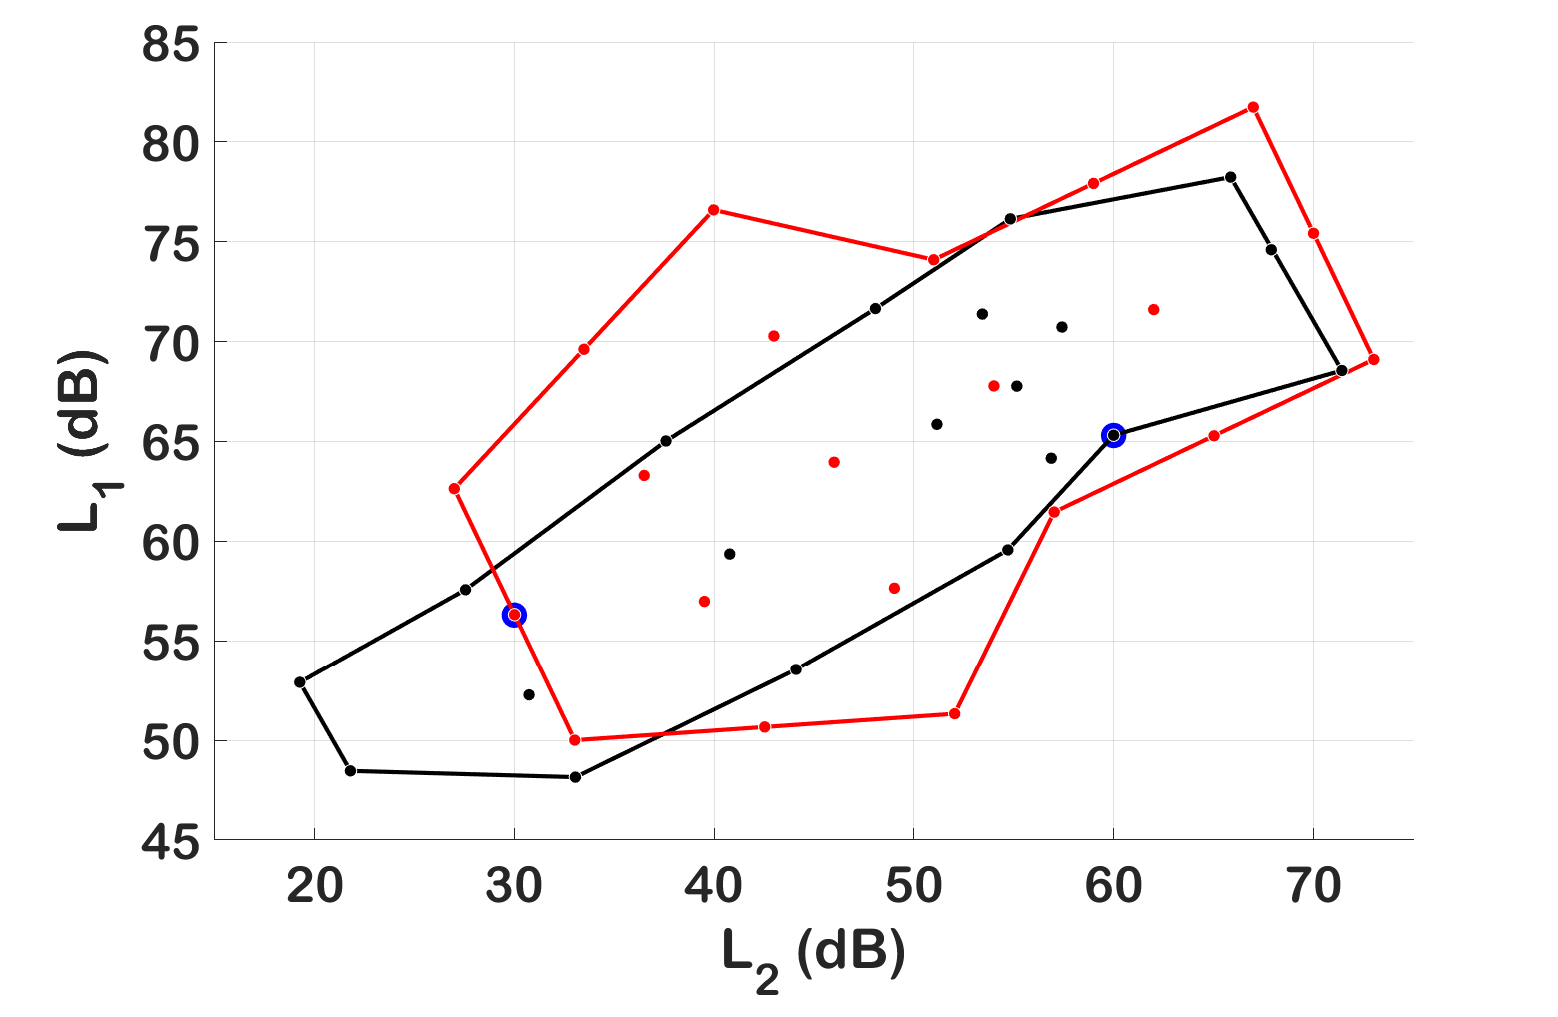
\includegraphics[width=\columnwidth]{Fig_3_connectivity.eps}}
\caption{Accepted points and their correspondent alpha shapes: adaptive (black) and static (red) level maps. Initial points for both approaches are highlighted with blue circles. An ideal scenario where all points meet the acceptance criteria, and the level maps do not clip to the ROI boundaries.}
\label{fig_CNT}
\end{figure}

Time efficiency of an LM measurement is defined here as the ratio of accepted points to all acquired points $(N_{acc}/N_{all})$. The second metric is used to assess a “goodness” of coverage. Together with $S$, the areal density of the points with accepted DPOAE amplitudes $(\rho = N_{acc} / S)$ creates a $(\rho, S)$-space, where the main underlying assumption is, that there exists an ideal LM with ideal values, i.e. $(\rho _{max}, S_{max})$, where $\rho _{max}$, $S_{max}$ are the maximum values of these variables across all LMs (here 6 ears x 14 frequencies x 2 methods). In this context, any reduction in Nacc leads to a value below one. Similarly, any dispersion over a larger area S in the $(L_2, L_1)$-plane leads to a value below one. The latter criterion $\rho < 1$  is here taken as an indicator of loss of information.

\subsubsection{Comparison of obtained maps}
First, the accepted points, acquired with SLM and ALM, are interpolated using biharmonic splines (X. Deng, Z. Tang, 2011). For ridge identification, the measured level map is transformed into a gradient field. A simplified version of the Dijkstra algorithm (Dijkstra, E.W., 1959) is used to trace the path with the least inclination from the peak towards lower values. The customized algorithm includes the following simplifications: it operates on a predefined mesh graph, only allows movement towards lower or equal $L_2$ values from the initial point,  has an open end instead of searching for a distant endpoint, and considers only neighbouring nodes of the mesh. To reduce oscillations and enhance stability, additional weighting is applied to the gradient field based on two rules: 1) nodes with $L_2$ lower than initial point and 2) nodes, which are closer to the line connecting the initial point to the closest local minimum on gradient field, have their weight partially increased. 

To compare LM shapes obtained via different methods, we need a common measure that incorporates all the evaluated data. 

This is achieved by applying a joint polynomial fit, where each estimated ridge is fitted to its own polynomial with $k$ characteristic low-order terms and iterative $n-k$ shared higher-order components. The order of the polynomial is incremented by 1 and is limited by $k = 1$, $n_{max} = 15$.


\begin{align}
\begin{cases}
p_{n} x_{\alpha}^n&+p_{n-1} x_{\alpha}^{n-1}+\cdots+p_{k+1} x_{\alpha}^{k+1} \\
&+\alpha_k x_{\alpha}^{k}+\alpha_{k-1} x_{\alpha}^{k-1}+\cdots+\alpha _0 x_{\alpha}^0-y_{\alpha} =0 \\
p_{n} x_{\beta}^n&+p_{n-1} x_{\beta}^{n-1}+\cdots+p_{k+1} x_{\beta}^{k+1} \\
&+\beta_k x_{\beta}^{k}+\beta_{k-1} x_{\beta}^{k-1}+\cdots+\beta _0 x_{\beta}^0-y_{\beta} =0 \\
& \vdots 
\end{cases}
\label{eq1}
\end{align}

The K-Fold cross-validation is used to prevent overfitting, where amount of folds is selected dynamically based on size of data (with minimum four and maximum ten folds). When one of the lines is considered to be overfitted, then previous state is taken as a result.

A common ridge is then determined by fitting the remaining free components using the previously identified higher-order terms. The final step is to calculate the distances of points to the joint fit of the ridges of SLM and ALM methods (see Fig. 5).

\section{Results}

\begin{figure*}
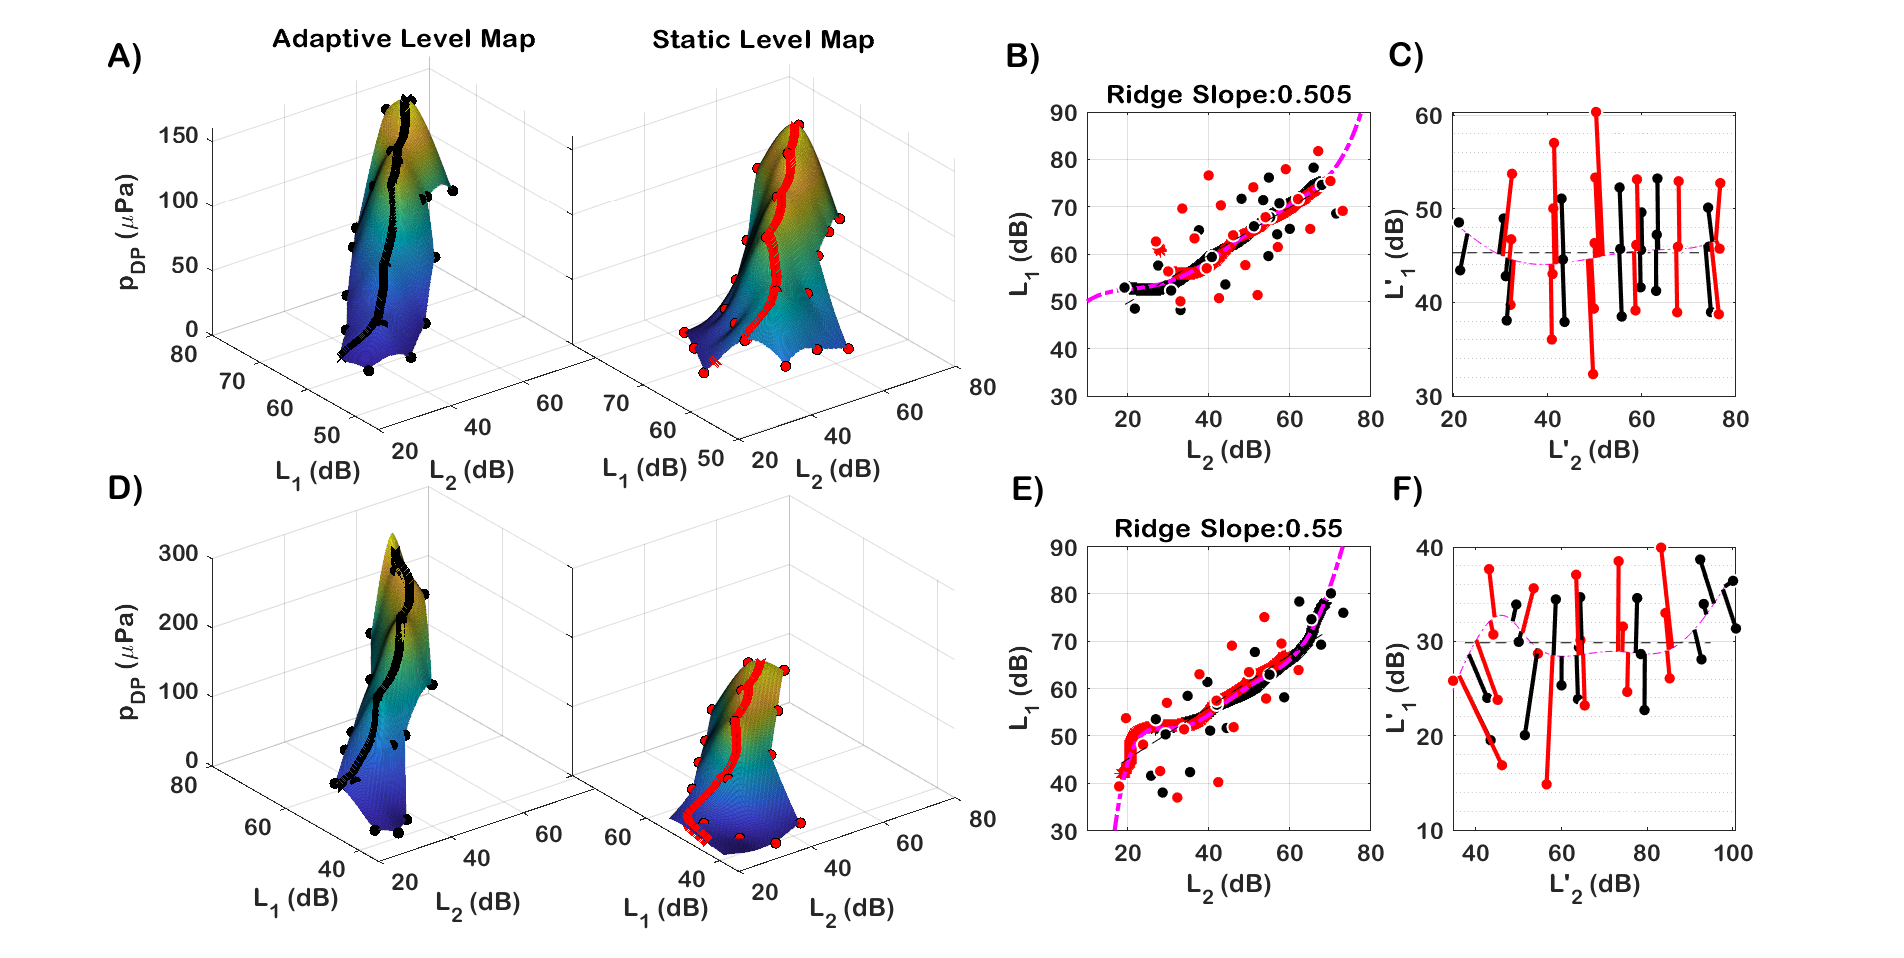
\includegraphics[width=\textwidth]{Fig_5_assembly2.eps} %,height=4cm
\caption{Features estimation routine: A, D) A level map interpolated with biharmonic splines and its ridge, estimated using the "ridge searcher" method. B, E) Estimated ridges from the LMs in A, D) and a general ridge derived through iterative polynomial fitting of these two ridges. C, F) Distances between the general ridge and measured points for both maps. A-C) represent a nearly ideal case (S345, 4 kHz), whereas D-F) show more common outcome of LM acquisition (S345, 2 kHz).\\ Black colour – Adaptive Level Map, Red colour – Static Level Map.}
\label{fig_BLK}
\end{figure*}

\subsection{Qualitative features of the interpolation and ridge comparison method}
Fig. 5A-C and Fig. 5D-F show two examples of LMs pairs obtained with the adaptive (black curve) and the static (red curve) method. The upper example (Fig. 5A) illustrates an acquisition of a nearly ideal level map. For both, the ALM and the SLM, all measured points met the SNR criterion (only points, passing the SNR criterion, are connected by the mesh illustrating the surface in (Fig. 5B)). The interpolation method used, introduces rippling along the ridge, which putatively does not reflect the true shape of the level map, and should be considered as an artefact resulting from limited sampling density. The black and the red line designate the result of the ridge search algorithm (see Section II.E). In this example (Fig. 5A-C), the ridge lines cut almost always through the central points accurately. 

A less favourable example with an irregular form of the level maps  is shown in Fig. 5D. Fig. 5B and E show the projection of the identified ridges and the stimulus level pairs of accepted points onto the $(L_2, L_1)$-plane. In an ideal case   the ridges of both, ALM and SLM, align closely and correspond to straight lines. However, in Fig. 5E,  the ridge identified for the SLM method is shifted toward lower $L_1$ values, intersecting only one experimentally measured point exactly, while, the ridge identified by the ALM method aligns more closely with the centre line of the acquisition. The projection of both ridge identifications onto the $(L_2, L_1)$-plane appears to comprise deviations from a straight line, although it is not completely clear to which extent the deviations are a result of the surface interpolation method.

\subsection{Time efficiency}
Fig. 6A shows the acceptance rate (Nacc/Nall), representing the portion of points that passed the $10 dB$ SNR criterion, across all six ears, dependent on frequency. In general, ALM measurements resulted in a greater number of accepted points at most frequencies, the exceptions being 3, 12, and 13 kHz. Fig.6B shows the histogram of the acceptance rate within a single LM across all frequencies and all ears. ALM show in $32\%$ of all LMs an acceptance rate of $\ge 0.95$, i.e. 20 out of 21 or all points which have been tested passed the SNR criterion, while the correspondent figure for SLM was only $11\%$. The median of the acceptance rate was 0.68 and 0.76 for SLM and ALM indicating that ALM is more effective in setting stimulus levels to achieve DPOAE signals with SNR $\ge10 dB$ compared to SLM.

\begin{figure}[ht]
\centerline{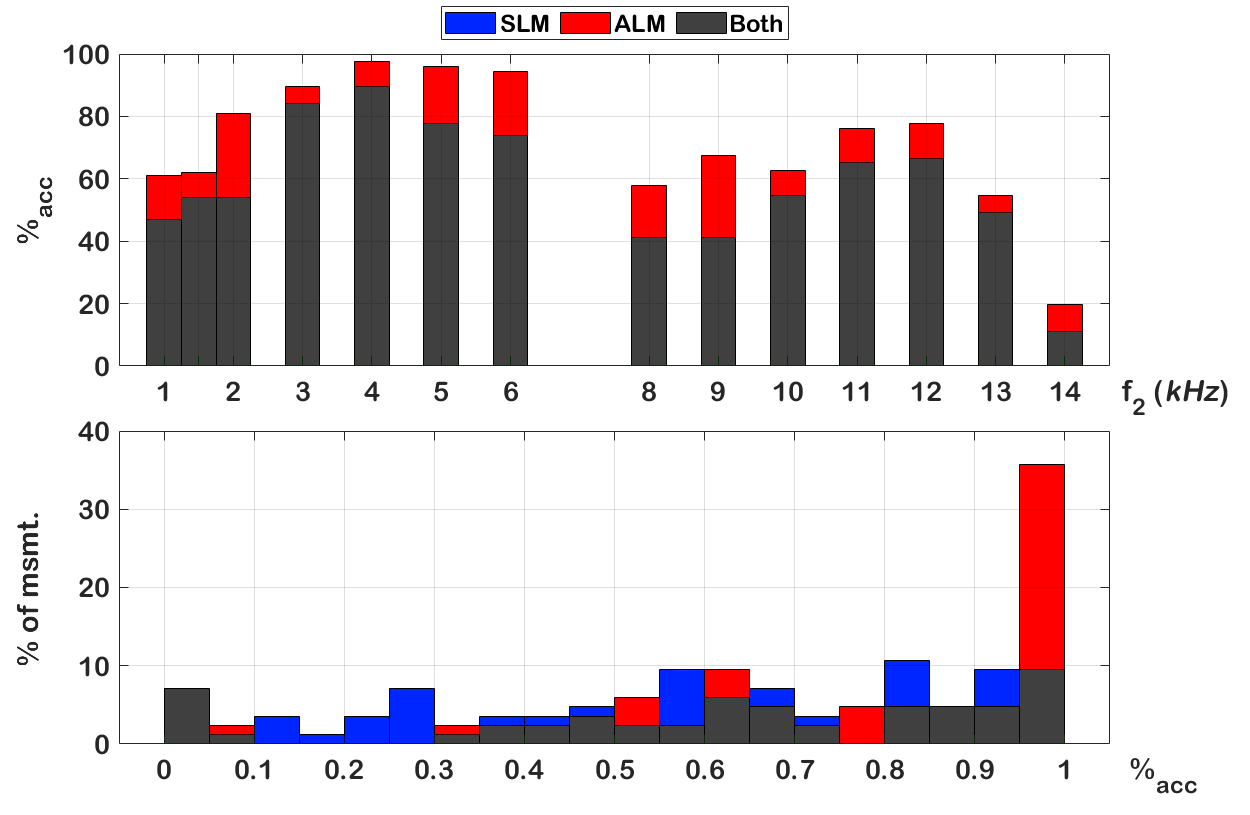
\includegraphics[width=\columnwidth]{Fig_Efficiency_v3.png}}
\caption{A) Share of accepted points over frequencies for all ears. B) Distribution of percentage of accepted points per single LM measurement for all frequencies and ears. Black color shows the method with the smaller or equal share .}
\label{fig_EFF}
\end{figure}

Overall, we obtained 1168 accepted DPOAE amplitudes with SLMs and 1312 accepted DPOAE amplitudes with ALMs, indicating a $12\%$ increase in quantitative output.

\subsection{Coverage of DPOAE LMs}
To compare the relative performance of both methods, we performed a joint analysis of the area, defined by the alpha shape corresponding to the accepted points, and their $(L_2, L_1)$-density (see Section II.E). Both values $(\rho, S)$ are min-max normalized in linear space and converted to log space (see Eq.2):
\begin{equation} log(\rho) = log(\frac{\rho - \rho_{min}}{\rho_{max} - \rho_{min}}); log(S) = log(\frac{S - S_{min}}{S_{max} - S_{min}}), \label{eq2}\end{equation}
where the minimum and maximum values are determined separately for each LM. Thus, in linear space, $\rho$ and $S$ cannot attain values of $> 1$, or equivalently their logarithm cannot become $> 0$. Therefore, a deviation of any of either parameters towards “$-\infty$” designates a loss of information.

\begin{figure*}
\centering
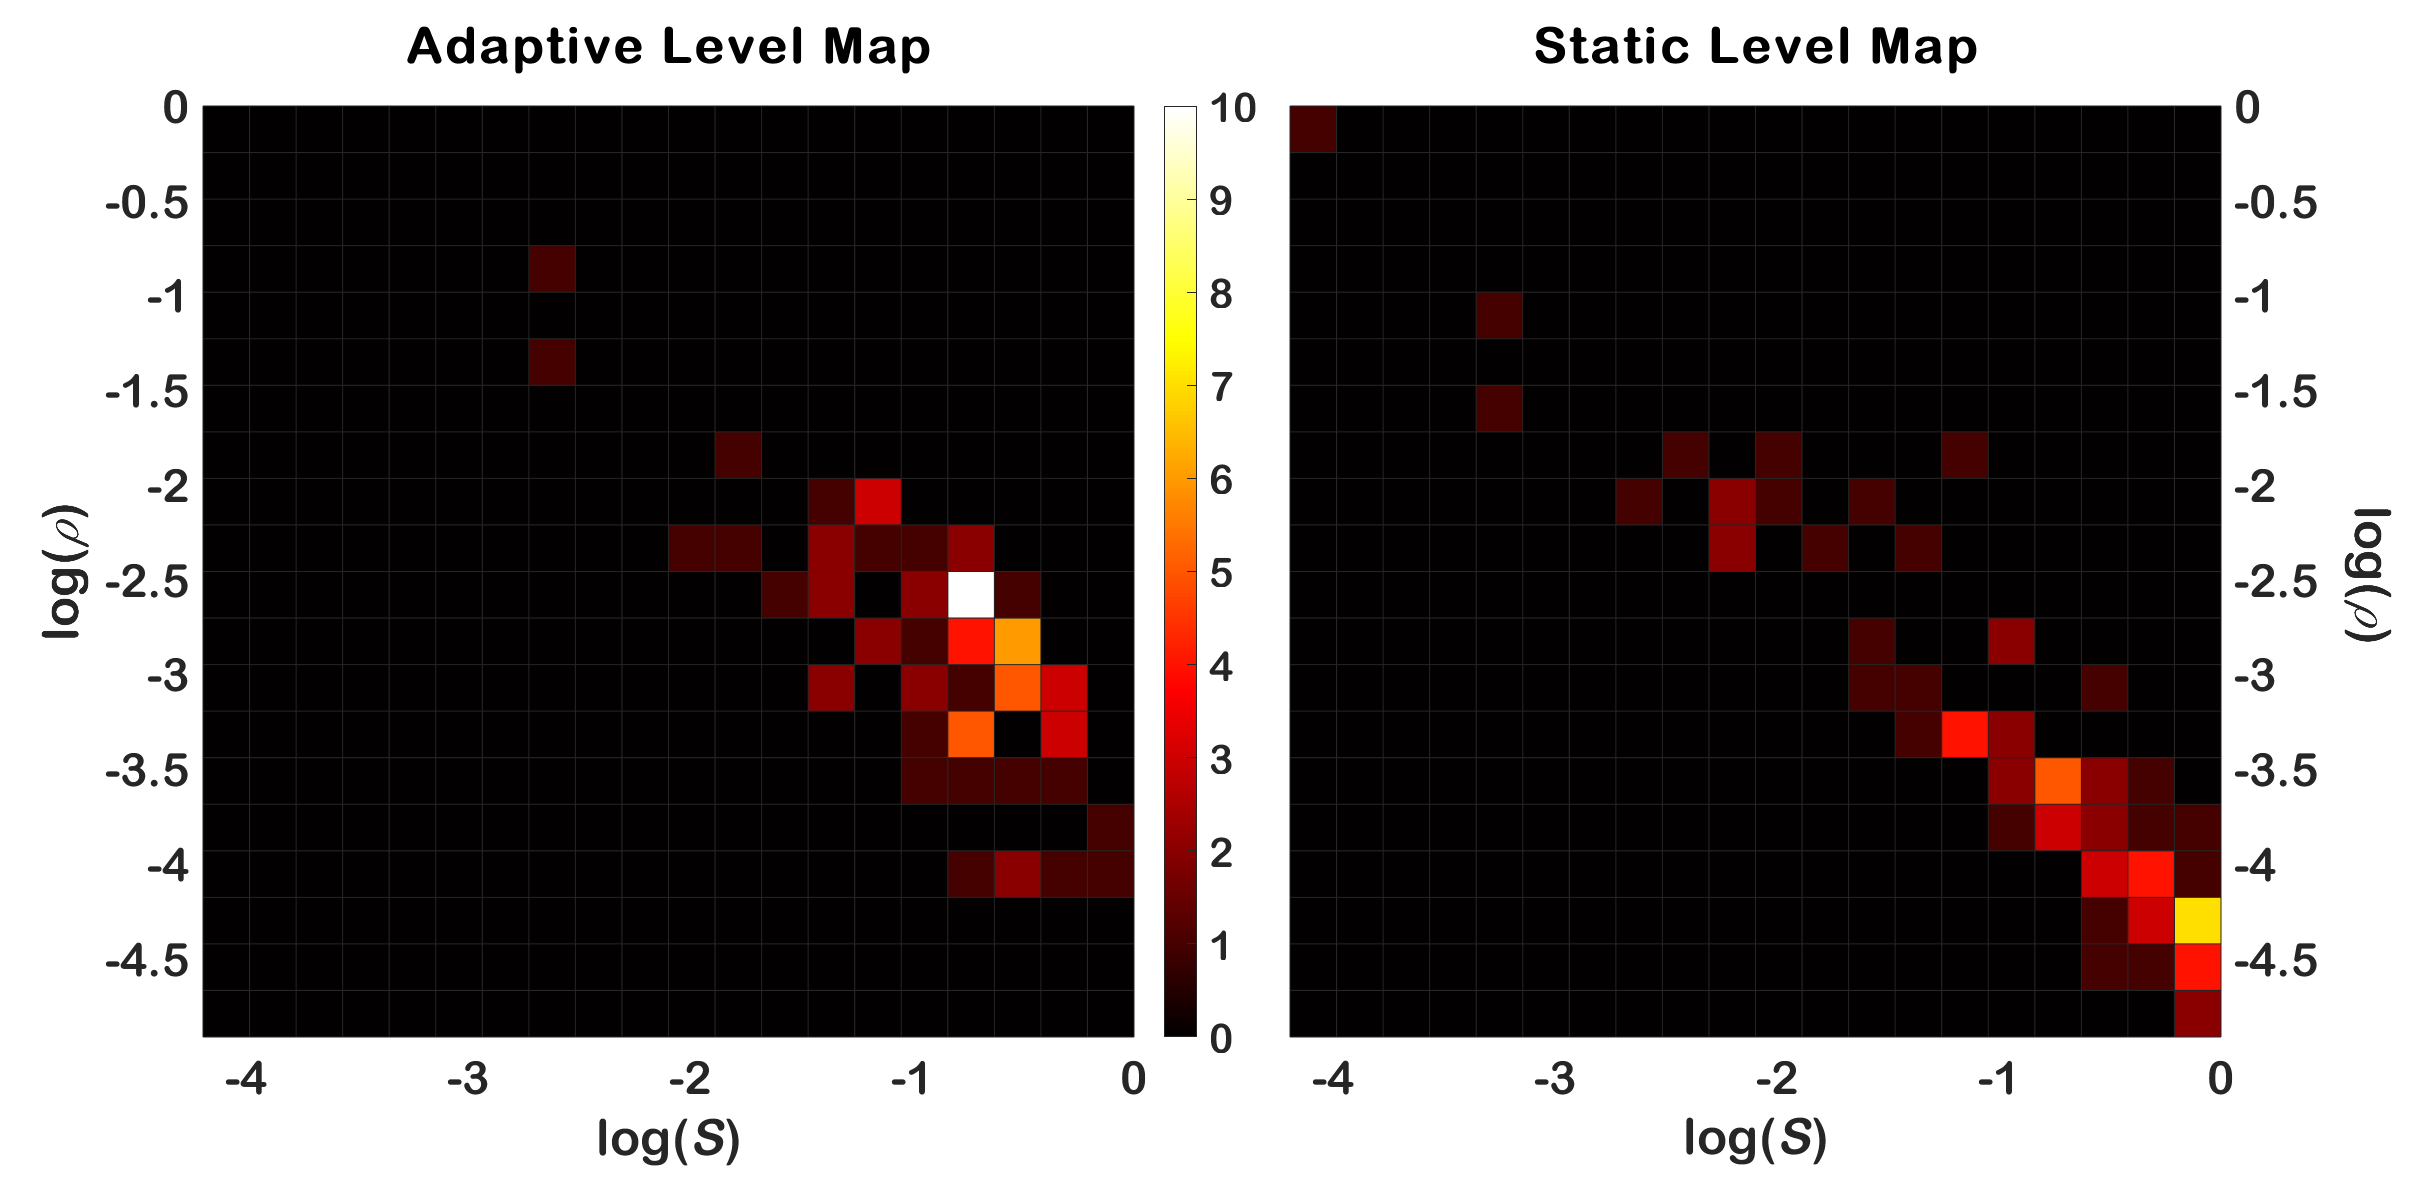
\includegraphics[width=.8\textwidth]{Fig_8_Coverage_sameClim.eps} %,height=4cm
\caption{Bivariate histogram of level map areas and their corresponding point density. This histogram is representing the qualitative aspect of LM properties which were encountered oin this study. There is an assumed ideal LM with largest area and density, which is located in $(0, 0)$, but cannot be obtained with the given amount of $N_{all}$. The colour scheme ranges from black through red to white. Higher colour intensity designates higher amount of counts.}
\label{fig_TGT}
\end{figure*}

Fig. 7 shows a bivariate histogram of area and density for the obtained level maps, with the left panel representing ALM, and the right panel representing SLM. The majority of measurements (clustered with brightest square as a centre) acquired with the ALM method is shifted towards $(0, 0)$, compared to those made with the SLM method. This shift suggests that ALMs prioritizes point density over area coverage, resulting in improved resolution.


\begin{figure}[ht]
\centerline{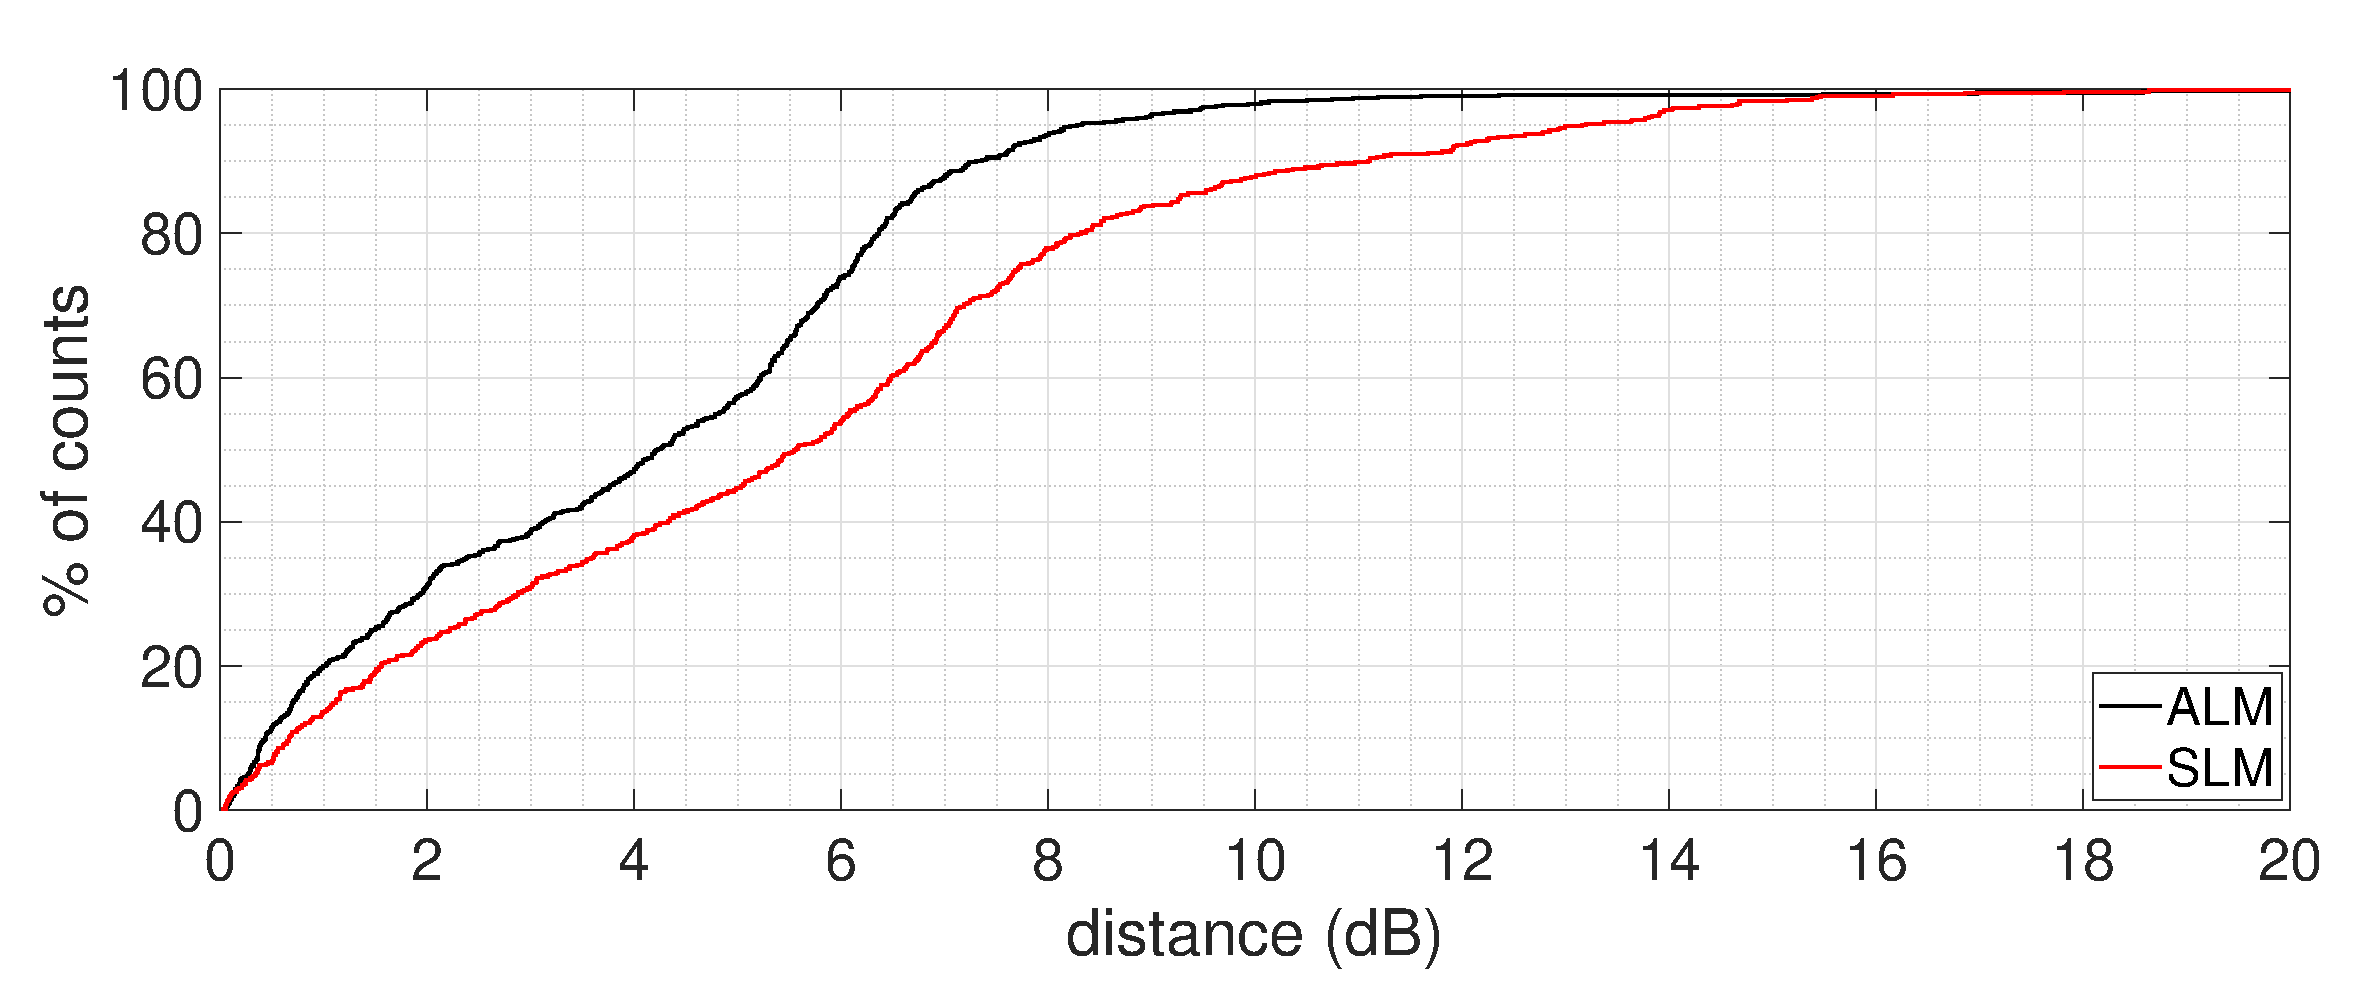
\includegraphics[width=\columnwidth]{Fig_9_Cumula.eps}}
\caption{Empirical cumulative distribution function of the distances between the estimated ridge and measured points.}
\label{fig_CDF}
\end{figure}

Fig. 8 shows the cumulative distribution of the distance of the (L1, L2)-coordinates of accepted points from the ridge. For ALM, 75\% of the accepted points lie within $6 dB$ from the ridge, compared to only 5\% for SLM. Moreover, in the static methods, more than 25\% of points are over $8 dB$ away from the ridge. Taking a typical level map cross section given by $L_{DP} =-0.12 \delta L_1^2$ (Eq. 4 and Tbl. I in Zelle, 2020), $8 dB$ off ridge suggests already a relative loss in SNR of $7.7 dB$, compared to only $4.3 dB$ for $6 dB$ distance.

\begin{figure}[ht]
\centerline{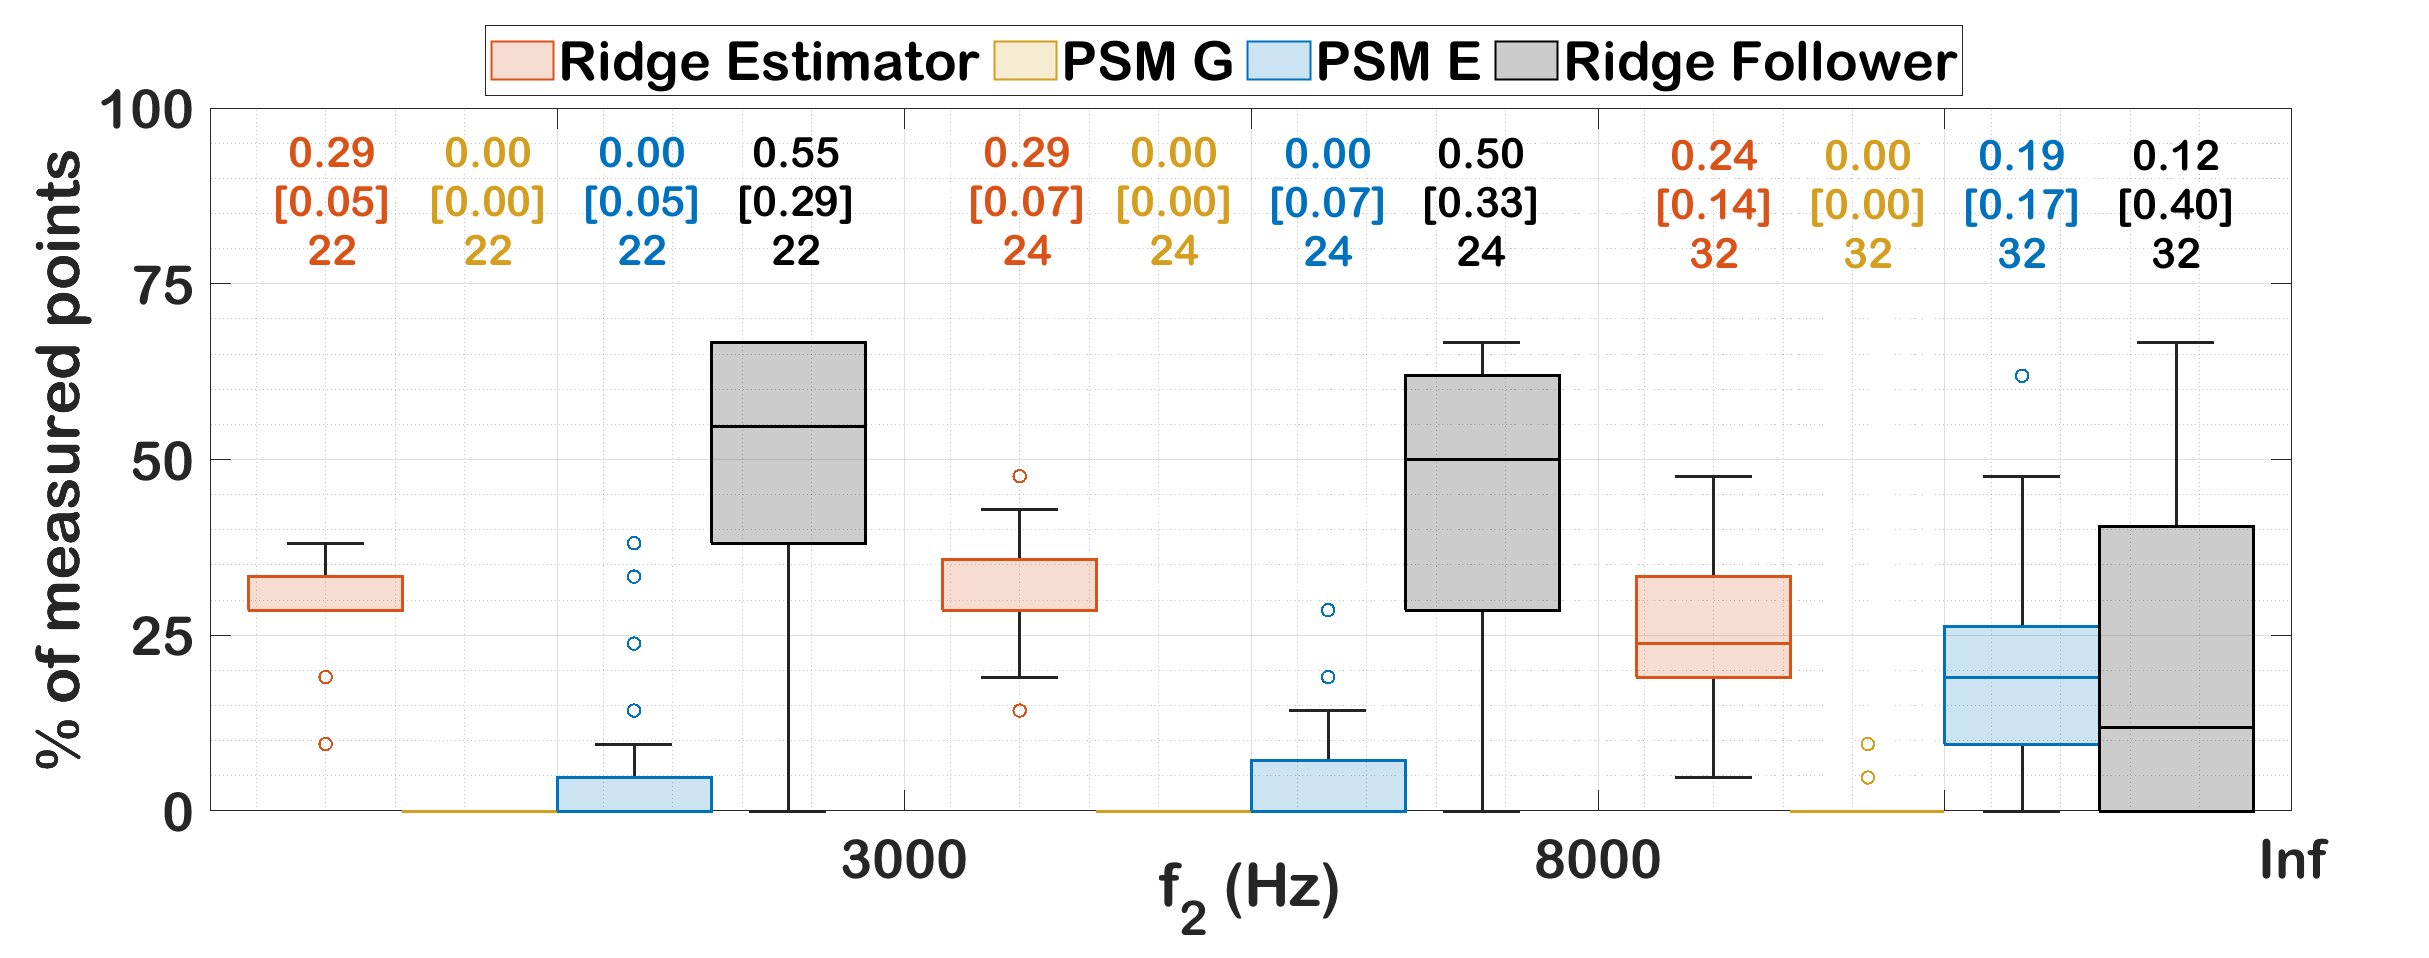
\includegraphics[width=\columnwidth]{Fig_10_Boxplots.eps}}
\caption{Median, interquartile ranges, and range of the share of accepted DPOAE within a level map due to the four adaptive acquisition methods, given for three frequency ranges.}
\label{fig_BXP}
\end{figure}

Fig. 9 shows the performance of the four adaptive acquisition methods in the implementation used here, give as statistics of the ratio of accepted points collected by a single method to all accepted points within a given LM (Formel). For the both lower frequency ranges, judged by the median, more than 80\% of the accepted points were successfully acquired by the a priori methods (ridge estimator and ridge follower), whereas the adaptive acquisition workflow (Fig. 3) only seldom needed to invoke the data-based algorithms. On the contrary, for the high-frequency range, as judged by the median, only 36\% of the accepted points were contributed by the a priori methods, whereas the data-based methods gained importance and contributed 19\%.

\section{Discussion}
This study pursued two major goals: First, design and approbate an adaptive level-map acquisition method that is able to prove the existence and sample the ridge. The second goal was to develop and investigate a method for characterization and comparison of all kind of level maps obtained by different methods without limiting them to a priori assumptions on their shape such as the 5-parameter model.

\subsection{Method advantages and drawbacks}
For various modalities (such as ultrasound, X-ray, microscopy, etc.), there are multiple techniques for processing data that is collected across different dimensions, with each dimension typically characterized by specific values (ISBN 978-3-319-96520-8 (eBook), https://doi.org/10.1007/978-3-319-96520-8).
While in most medical imaging systems, the measured value is typically defined by its spatial properties and multiple points being measured simultaneously, in DPOAE-acquisition the position of the acquired acoustic response is defined with $(L_2, L_1)$ stimulus level space and only a single point is being measured at a time to prevent technical distortions coming from the speaker.
Strictly speaking, adaptive methods are designed to extract features from the resulting LM while working with an extremely limited number of points. To address this, we employed a two-stage search sequence, consisting of pattern recognition (a priori) and exploratory (data-based) methods. While the idea behind the first group of methods is to recognize the single peak structure, the behaviour of exploratory method is a bit more complicated. These methods are applied when the required feature cannot be recognized using the ridge estimator method. Their concept is similar to the one shown in (Fig 1A-B, Chiang, J. Y, 1997), where the sampling grid covers the entire image and then becomes finer in areas to capture the feature more accurately.
Although these methods differ in their implementation and execution, they share a common structure and topology. At the core of the pattern recognition method is a simplified beta skeleton of the $(L_2, L_1, p_{DP})$-surface, a subset of the Delaunay triangulation that can be reconstructed into a polygonal surface (Eppstein, 1998).
This dynamic approach allowed us to improve the accuracy of predicted points, resulting in both overall and measurement-specific time efficiency increase (Fig. 6). At certain frequencies where SPL calibration is prone to resonance (e.g., 3, 12, and 13 kHz), a specific event occurs. As the maximum level values of the ROI decrease, SLMs struggle to adapt to these changes and measure strictly at the ROI boundary. In contrast, ALMs reassess the situation and attempt to gather the maximum amount of information given the new conditions. As a result, we observe a slight drop in the acceptance rate at these frequencies.
However ALM methods also have notable drawbacks. The most prominent one is bound to the limited number of points and our inclusion criteria (“accepted points”) – our methods are highly sensitive to false detections and technical distortions that might occur during measurement. False accepted points can lead algorithms off track and prevent them from efficiently capturing the feature. A second drawback is specific to PSM and arises from simplicity of our inclusion criteria. Accepted points is a binary state and does not fully account for the 3rd dimension, which means, that expansion case of PSM might get stuck in situations, when it measures a lot of low amplitude points and spends less time on feature acquisition.

\subsection{Time concern}
Partially, both goals stand in conflict, because the primary adaptive methods, i.e. ridge estimator and ridge follower, rely on the a-priori assumption that a physiologically healthy cochlea presents a level map having a certain ridge structure. Also, before delving into a detailed discussion, it is instructive to consider that in a routine clinical application, more than some 7 to 9 points per level map will probably be undesirable, because with a typical amount of 6–8 test frequencies, extrapolation of the figures given in Sec. II.C would lead to a measurement time of 3min35' to 6min8' in the current implementation. According to our estimation, by additional optimization of the implementation, the measurement time could be reduced to below 3–4 min, what would be clinically attractive. If we consider a basic research aim as, for instance, the characterization of the deviation of individual level maps from the simplified 5-p model and/or the characterization of its time invariance, one easily end up with substantial measurements times, even if it is performed with an adaptive method.

\subsection{LM post-processing and analysis}
To analyse LMs of different origins, we devised a specific toolset that does not impose a priori assumptions and relies on spline interpolation, which is based solely on the acquired points and equations (X. Deng, 2011). As shown on Fig.5, a significant share (\#number!!!) of LMs recorded in normal hearing subjects meets the criteria for a good fit with proposed model function (Zelle 2020), given in (Section II D). This allows us to extract the ridge as a feature of the measured LMs use it as the reference, when comparing the acquired surfaces. The ALM methods have shown significantly better result in terms of resolution across the ridge (Fig. 8). One might argue, that this is a sort of self-fulfilling prophecy, since the 5-p model is used for point prediction. However, on the other hand, this shape is a well-established pattern (Whitehead, Zelle, …) that our methods have successfully assessed, which was one of initial reasons for their creation.

\section{Conclusion (SKETCH) (WORDS LIMIT = 300)}
Text

\section{Template}

\subsection{Equations}
Use one space after periods and colons. Hyphenate complex modifiers: 
``zero-field-cooled magnetization.'' Avoid dangling participles, such as, 
``Using \eqref{eq}, the potential was calculated.'' [It is not clear who or what 
used \eqref{eq}.] Write instead, ``The potential was calculated by using \eqref{eq},'' or 
``Using \eqref{eq}, we calculated the potential.''

Use a zero before decimal points: ``0.25,'' not ``.25.'' Use 
``cm$^{3}$,'' not ``cc.'' Indicate sample dimensions as ``0.1 cm 
$\times $ 0.2 cm,'' not ``0.1 $\times $ 0.2 cm$^{2}$.'' The 
abbreviation for ``seconds'' is ``s,'' not ``sec.'' Use 
``Wb/m$^{2}$'' or ``webers per square meter,'' not 
``webers/m$^{2}$.'' When expressing a range of values, write ``7 to 
9'' or ``7--9,'' not ``7$\sim $9.''

A parenthetical statement at the end of a sentence is punctuated outside of 
the closing parenthesis (like this). (A parenthetical sentence is punctuated 
within the parentheses.) In American English, periods and commas are within 
quotation marks, like ``this period.'' Other punctuation is ``outside''! 
Avoid contractions; for example, write ``do not'' instead of ``don't.'' The 
serial comma is preferred: ``A, B, and C'' instead of ``A, B and C.''

If you wish, you may write in the first person singular or plural and use 
the active voice (``I observed that $\ldots$'' or ``We observed that $\ldots$'' 
instead of ``It was observed that $\ldots$''). Remember to check spelling. If 
your native language is not English, please get a native English-speaking 
colleague to carefully proofread your paper.

Try not to use too many typefaces in the same article. You're writing
scholarly papers, not ransom notes. Also please remember that MathJax
can't handle really weird typefaces.

Number equations consecutively with equation numbers in parentheses flush 
with the right margin, as in \eqref{eq}. To make your equations more 
compact, you may use the solidus (~/~), the exp function, or appropriate 
exponents. Use parentheses to avoid ambiguities in denominators. Punctuate 
equations when they are part of a sentence, as in
\begin{equation}E=mc^2.\label{eq}\end{equation}

Be sure that the symbols in your equation have been defined before the 
equation appears or immediately following. Italicize symbols ($T$ might refer 
to temperature, but T is the unit tesla). Refer to ``\eqref{eq},'' not ``Eq. \eqref{eq}'' 
or ``equation \eqref{eq},'' except at the beginning of a sentence: ``Equation \eqref{eq} 
is $\ldots$ .''

\subsection{\LaTeX-Specific Advice}

Please use ``soft'' (e.g., \verb|\eqref{Eq}|) cross references instead
of ``hard'' references (e.g., \verb|(1)|). That will make it possible
to combine sections, add equations, or change the order of figures or
citations without having to go through the file line by line.

Please don't use the \verb|{eqnarray}| equation environment. Use
\verb|{align}| or \verb|{IEEEeqnarray}| instead. The \verb|{eqnarray}|
environment leaves unsightly spaces around relation symbols.

Please note that the \verb|{subequations}| environment in {\LaTeX}
will increment the main equation counter even when there are no
equation numbers displayed. If you forget that, you might write an
article in which the equation numbers skip from (17) to (20), causing
the copy editors to wonder if you've discovered a new method of
counting.

{\BibTeX} does not work by magic. It doesn't get the bibliographic
data from thin air but from .bib files. If you use {\BibTeX} to produce a
bibliography you must send the .bib files. 

{\LaTeX} can't read your mind. If you assign the same label to a
subsubsection and a table, you might find that Table I has been cross
referenced as Table IV-B3. 

{\LaTeX} does not have precognitive abilities. If you put a
\verb|\label| command before the command that updates the counter it's
supposed to be using, the label will pick up the last counter to be
cross referenced instead. In particular, a \verb|\label| command
should not go before the caption of a figure or a table.

Do not use \verb|\nonumber| inside the \verb|{array}| environment. It
will not stop equation numbers inside \verb|{array}| (there won't be
any anyway) and it might stop a wanted equation number in the
surrounding equation.

If you are submitting your paper to a colorized journal, you can use
the following two lines at the start of the article to ensure its
appearance resembles the final copy:

\smallskip\noindent
\begin{small}
\begin{tabular}{l}
\verb+\+\texttt{documentclass[journal,twoside,web]\{ieeecolor\}}\\
\verb+\+\texttt{usepackage\{\textit{Journal\_Name}\}}
\end{tabular}
\end{small}

The SI unit for magnetic field strength $H$ is A/m. However, if you wish to use 
units of T, either refer to magnetic flux density $B$ or magnetic field 
strength symbolized as $\mu _{0}H$. Use the center dot to separate 
compound units, e.g., ``A$\cdot $m$^{2}$.''

The word ``data'' is plural, not singular. The subscript for the 
permeability of vacuum $\mu _{0}$ is zero, not a lowercase letter 
``o.'' The term for residual magnetization is ``remanence''; the adjective 
is ``remanent''; do not write ``remnance'' or ``remnant.'' Use the word 
``micrometer'' instead of ``micron.'' A graph within a graph is an 
``inset,'' not an ``insert.'' The word ``alternatively'' is preferred to the 
word ``alternately'' (unless you really mean something that alternates). Use 
the word ``whereas'' instead of ``while'' (unless you are referring to 
simultaneous events). Do not use the word ``essentially'' to mean 
``approximately'' or ``effectively.'' Do not use the word ``issue'' as a 
euphemism for ``problem.'' When compositions are not specified, separate 
chemical symbols by en-dashes; for example, ``NiMn'' indicates the 
intermetallic compound Ni$_{0.5}$Mn$_{0.5}$ whereas 
``Ni--Mn'' indicates an alloy of some composition 
Ni$_{x}$Mn$_{1-x}$.

\begin{figure}[!t]
\centerline{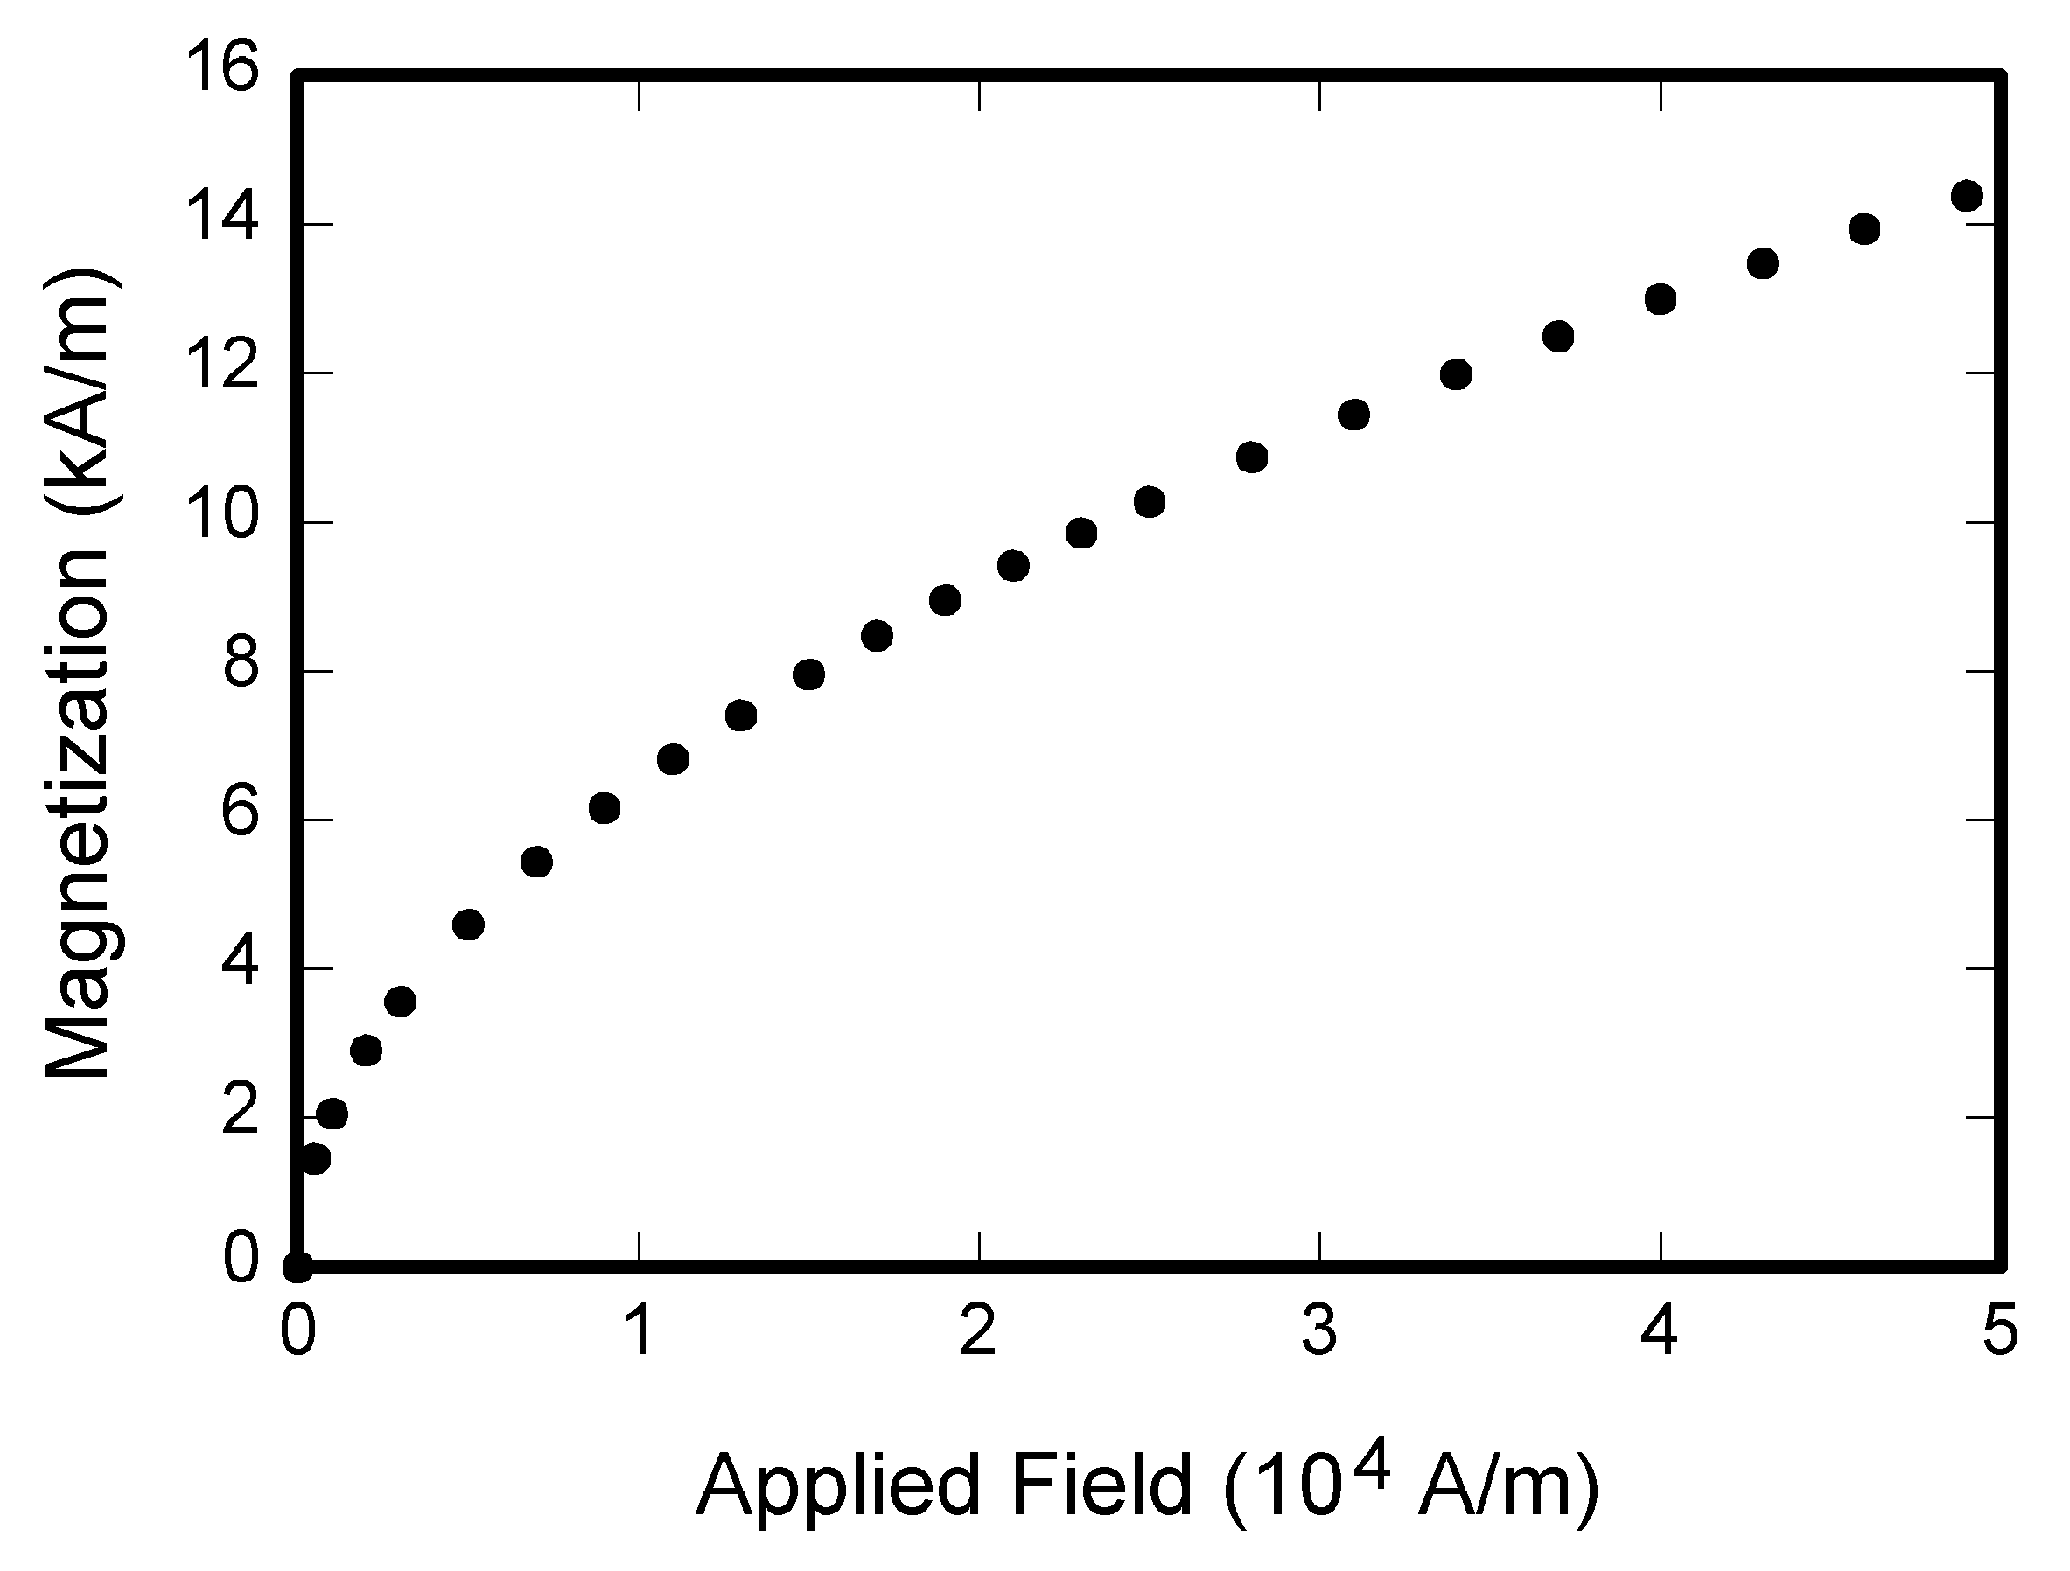
\includegraphics[width=\columnwidth]{fig1.png}}
\caption{Magnetization as a function of applied field.
It is good practice to explain the significance of the figure in the caption.}
\label{fig1}
\end{figure}

Be aware of the different meanings of the homophones ``affect'' (usually a 
verb) and ``effect'' (usually a noun), ``complement'' and ``compliment,'' 
``discreet'' and ``discrete,'' ``principal'' (e.g., ``principal 
investigator'') and ``principle'' (e.g., ``principle of measurement''). Do 
not confuse ``imply'' and ``infer.'' 

Prefixes such as ``non,'' ``sub,'' ``micro,'' ``multi,'' and ``ultra'' are 
not independent words; they should be joined to the words they modify, 
usually without a hyphen. There is no period after the ``et'' in the Latin 
abbreviation ``\emph{et al.}'' (it is also italicized). The abbreviation ``i.e.,'' means 
``that is,'' and the abbreviation ``e.g.,'' means ``for example'' (these 
abbreviations are not italicized).

A general IEEE styleguide is available at \underline{http://www.ieee.org/authortools}.

\section{Guidelines for Graphics Preparation and Submission}
\label{sec:guidelines}

\subsection{Types of Graphics}
The following list outlines the different types of graphics published in 
IEEE journals. They are categorized based on their construction, and use of 
color/shades of gray:

\subsubsection{Color/Grayscale figures}
{Figures that are meant to appear in color, or shades of black/gray. Such 
figures may include photographs, illustrations, multicolor graphs, and 
flowcharts.}

\subsubsection{Line Art figures}
{Figures that are composed of only black lines and shapes. These figures 
should have no shades or half-tones of gray, only black and white.}

\subsubsection{Author photos}
{Head and shoulders shots of authors that appear at the end of our papers. }

\subsubsection{Tables}
{Data charts which are typically black and white, but sometimes include 
color.}

\begin{table}
\caption{Units for Magnetic Properties}
\label{table}
\setlength{\tabcolsep}{3pt}
\begin{tabular}{|p{25pt}|p{75pt}|p{115pt}|}
\hline
Symbol& 
Quantity& 
Conversion from Gaussian and \par CGS EMU to SI $^{\mathrm{a}}$ \\
\hline
$\Phi $& 
magnetic flux& 
1 Mx $\to  10^{-8}$ Wb $= 10^{-8}$ V$\cdot $s \\
$B$& 
magnetic flux density, \par magnetic induction& 
1 G $\to  10^{-4}$ T $= 10^{-4}$ Wb/m$^{2}$ \\
$H$& 
magnetic field strength& 
1 Oe $\to  10^{3}/(4\pi )$ A/m \\
$m$& 
magnetic moment& 
1 erg/G $=$ 1 emu \par $\to 10^{-3}$ A$\cdot $m$^{2} = 10^{-3}$ J/T \\
$M$& 
magnetization& 
1 erg/(G$\cdot $cm$^{3}) =$ 1 emu/cm$^{3}$ \par $\to 10^{3}$ A/m \\
4$\pi M$& 
magnetization& 
1 G $\to  10^{3}/(4\pi )$ A/m \\
$\sigma $& 
specific magnetization& 
1 erg/(G$\cdot $g) $=$ 1 emu/g $\to $ 1 A$\cdot $m$^{2}$/kg \\
$j$& 
magnetic dipole \par moment& 
1 erg/G $=$ 1 emu \par $\to 4\pi \times  10^{-10}$ Wb$\cdot $m \\
$J$& 
magnetic polarization& 
1 erg/(G$\cdot $cm$^{3}) =$ 1 emu/cm$^{3}$ \par $\to 4\pi \times  10^{-4}$ T \\
$\chi , \kappa $& 
susceptibility& 
1 $\to  4\pi $ \\
$\chi_{\rho }$& 
mass susceptibility& 
1 cm$^{3}$/g $\to  4\pi \times  10^{-3}$ m$^{3}$/kg \\
$\mu $& 
permeability& 
1 $\to  4\pi \times  10^{-7}$ H/m \par $= 4\pi \times  10^{-7}$ Wb/(A$\cdot $m) \\
$\mu_{r}$& 
relative permeability& 
$\mu \to \mu_{r}$ \\
$w, W$& 
energy density& 
1 erg/cm$^{3} \to  10^{-1}$ J/m$^{3}$ \\
$N, D$& 
demagnetizing factor& 
1 $\to  1/(4\pi )$ \\
\hline
\multicolumn{3}{p{251pt}}{Vertical lines are optional in tables. Statements that serve as captions for 
the entire table do not need footnote letters. }\\
\multicolumn{3}{p{251pt}}{$^{\mathrm{a}}$Gaussian units are the same as cg emu for magnetostatics; Mx 
$=$ maxwell, G $=$ gauss, Oe $=$ oersted; Wb $=$ weber, V $=$ volt, s $=$ 
second, T $=$ tesla, m $=$ meter, A $=$ ampere, J $=$ joule, kg $=$ 
kilogram, H $=$ henry.}
\end{tabular}
\label{tab1}
\end{table}

\subsection{Multipart figures}
Figures compiled of more than one sub-figure presented side-by-side, or 
stacked. If a multipart figure is made up of multiple figure
types (one part is lineart, and another is grayscale or color) the figure 
should meet the stricter guidelines.

\subsection{File Formats For Graphics}\label{formats}
Format and save your graphics using a suitable graphics processing program 
that will allow you to create the images as PostScript (PS), Encapsulated 
PostScript (.EPS), Tagged Image File Format (.TIFF), Portable Document 
Format (.PDF), Portable Network Graphics (.PNG), or Metapost (.MPS), sizes them, and adjusts 
the resolution settings. When 
submitting your final paper, your graphics should all be submitted 
individually in one of these formats along with the manuscript.

\subsection{Sizing of Graphics}
Most charts, graphs, and tables are one column wide (3.5 inches/88 
millimeters/21 picas) or page wide (7.16 inches/181 millimeters/43 
picas). The maximum depth a graphic can be is 8.5 inches (216 millimeters/54
picas). When choosing the depth of a graphic, please allow space for a 
caption. Figures can be sized between column and page widths if the author 
chooses, however it is recommended that figures are not sized less than 
column width unless when necessary. 

There is currently one publication with column measurements that do not 
coincide with those listed above. Proceedings of the IEEE has a column 
measurement of 3.25 inches (82.5 millimeters/19.5 picas). 

The final printed size of author photographs is exactly
1 inch wide by 1.25 inches tall (25.4 millimeters$\,\times\,$31.75 millimeters/6 
picas$\,\times\,$7.5 picas). Author photos printed in editorials measure 1.59 inches 
wide by 2 inches tall (40 millimeters$\,\times\,$50 millimeters/9.5 picas$\,\times\,$12 
picas).

\subsection{Resolution }
The proper resolution of your figures will depend on the type of figure it 
is as defined in the ``Types of Figures'' section. Author photographs, 
color, and grayscale figures should be at least 300dpi. Line art, including 
tables should be a minimum of 600dpi.

\subsection{Vector Art}
In order to preserve the figures' integrity across multiple computer 
platforms, we accept files in the following formats: .EPS/.PDF/.PS. All 
fonts must be embedded or text converted to outlines in order to achieve the 
best-quality results.

\subsection{Color Space}
The term color space refers to the entire sum of colors that can be 
represented within the said medium. For our purposes, the three main color 
spaces are Grayscale, RGB (red/green/blue) and CMYK 
(cyan/magenta/yellow/black). RGB is generally used with on-screen graphics, 
whereas CMYK is used for printing purposes.

All color figures should be generated in RGB or CMYK color space. Grayscale 
images should be submitted in Grayscale color space. Line art may be 
provided in grayscale OR bitmap colorspace. Note that ``bitmap colorspace'' 
and ``bitmap file format'' are not the same thing. When bitmap color space 
is selected, .TIF/.TIFF/.PNG are the recommended file formats.

\subsection{Accepted Fonts Within Figures}
When preparing your graphics IEEE suggests that you use of one of the 
following Open Type fonts: Times New Roman, Helvetica, Arial, Cambria, and 
Symbol. If you are supplying EPS, PS, or PDF files all fonts must be 
embedded. Some fonts may only be native to your operating system; without 
the fonts embedded, parts of the graphic may be distorted or missing.

A safe option when finalizing your figures is to strip out the fonts before 
you save the files, creating ``outline'' type. This converts fonts to 
artwork what will appear uniformly on any screen.

\subsection{Using Labels Within Figures}

\subsubsection{Figure Axis labels }
Figure axis labels are often a source of confusion. Use words rather than 
symbols. As an example, write the quantity ``Magnetization,'' or 
``Magnetization M,'' not just ``M.'' Put units in parentheses. Do not label 
axes only with units. As in Fig. 1, for example, write ``Magnetization 
(A/m)'' or ``Magnetization (A$\cdot$m$^{-1}$),'' not just ``A/m.'' Do not label axes with a ratio of quantities and 
units. For example, write ``Temperature (K),'' not ``Temperature/K.'' 

Multipliers can be especially confusing. Write ``Magnetization (kA/m)'' or 
``Magnetization (10$^{3}$ A/m).'' Do not write ``Magnetization 
(A/m)$\,\times\,$1000'' because the reader would not know whether the top 
axis label in Fig. 1 meant 16000 A/m or 0.016 A/m. Figure labels should be 
legible, approximately 8 to 10 point type.

\subsubsection{Subfigure Labels in Multipart Figures and Tables}
Multipart figures should be combined and labeled before final submission. 
Labels should appear centered below each subfigure in 8 point Times New 
Roman font in the format of (a) (b) (c). 

\subsection{File Naming}
Figures (line artwork or photographs) should be named starting with the 
first 5 letters of the author's last name. The next characters in the 
filename should be the number that represents the sequential 
location of this image in your article. For example, in author 
``Anderson's'' paper, the first three figures would be named ander1.tif, 
ander2.tif, and ander3.ps.

Tables should contain only the body of the table (not the caption) and 
should be named similarly to figures, except that `.t' is inserted 
in-between the author's name and the table number. For example, author 
Anderson's first three tables would be named ander.t1.tif, ander.t2.ps, 
ander.t3.eps.

Author photographs should be named using the first five characters of the 
pictured author's last name. For example, four author photographs for a 
paper may be named: oppen.ps, moshc.tif, chen.eps, and duran.pdf.

If two authors or more have the same last name, their first initial(s) can 
be substituted for the fifth, fourth, third$\ldots$ letters of their surname 
until the degree where there is differentiation. For example, two authors 
Michael and Monica Oppenheimer's photos would be named oppmi.tif, and 
oppmo.eps.

\subsection{Referencing a Figure or Table Within Your Paper}
When referencing your figures and tables within your paper, use the 
abbreviation ``Fig.'' even at the beginning of a sentence. Do not abbreviate 
``Table.'' Tables should be numbered with Roman Numerals.

\subsection{Checking Your Figures: The IEEE Graphics Analyzer}
The IEEE Graphics Analyzer enables authors to pre-screen their graphics for 
compliance with IEEE Transactions and Journals standards before submission. 
The online tool, located at
\underline{http://graphicsqc.ieee.org/}, allows authors to 
upload their graphics in order to check that each file is the correct file 
format, resolution, size and colorspace; that no fonts are missing or 
corrupt; that figures are not compiled in layers or have transparency, and 
that they are named according to the IEEE Transactions and Journals naming 
convention. At the end of this automated process, authors are provided with 
a detailed report on each graphic within the web applet, as well as by 
email.

For more information on using the Graphics Analyzer or any other graphics 
related topic, contact the IEEE Graphics Help Desk by e-mail at 
graphics@ieee.org.

\subsection{Submitting Your Graphics}
Because IEEE will do the final formatting of your paper,
you do not need to position figures and tables at the top and bottom of each 
column. In fact, all figures, figure captions, and tables can be placed at 
the end of your paper. In addition to, or even in lieu of submitting figures 
within your final manuscript, figures should be submitted individually, 
separate from the manuscript in one of the file formats listed above in 
Section \ref{formats}. Place figure captions below the figures; place table titles 
above the tables. Please do not include captions as part of the figures, or 
put them in ``text boxes'' linked to the figures. Also, do not place borders 
around the outside of your figures.

\subsection{Color Processing/Printing in IEEE Journals}
All IEEE Transactions, Journals, and Letters allow an author to publish 
color figures on IEEE Xplore\textregistered\ at no charge, and automatically 
convert them to grayscale for print versions. In most journals, figures and 
tables may alternatively be printed in color if an author chooses to do so. 
Please note that this service comes at an extra expense to the author. If 
you intend to have print color graphics, include a note with your final 
paper indicating which figures or tables you would like to be handled that 
way, and stating that you are willing to pay the additional fee.

\section{Conclusion}
A conclusion section is not required. Although a conclusion may review the 
main points of the paper, do not replicate the abstract as the conclusion. A 
conclusion might elaborate on the importance of the work or suggest 
applications and extensions. 

\appendices

Appendixes, if needed, appear before the acknowledgment.

\section*{Acknowledgment}

The preferred spelling of the word ``acknowledgment'' in American English is 
without an ``e'' after the ``g.'' Use the singular heading even if you have 
many acknowledgments. Avoid expressions such as ``One of us (S.B.A.) would 
like to thank $\ldots$ .'' Instead, write ``F. A. Author thanks $\ldots$ .'' In most 
cases, sponsor and financial support acknowledgments are placed in the 
unnumbered footnote on the first page, not here.

\section*{References and Footnotes}

\subsection{References}
References need not be cited in text. When they are, they appear on the 
line, in square brackets, inside the punctuation. Multiple references are 
each numbered with separate brackets. When citing a section in a book, 
please give the relevant page numbers. In text, refer simply to the 
reference number. Do not use ``Ref.'' or ``reference'' except at the 
beginning of a sentence: ``Reference \cite{b3} shows $\ldots$ .'' Please do not use 
automatic endnotes in \emph{Word}, rather, type the reference list at the end of the 
paper using the ``References'' style.

Reference numbers are set flush left and form a column of their own, hanging 
out beyond the body of the reference. The reference numbers are on the line, 
enclosed in square brackets. In all references, the given name of the author 
or editor is abbreviated to the initial only and precedes the last name. Use 
them all; use \emph{et al.} only if names are not given. Use commas around Jr., 
Sr., and III in names. Abbreviate conference titles. When citing IEEE 
transactions, provide the issue number, page range, volume number, year, 
and/or month if available. When referencing a patent, provide the day and 
the month of issue, or application. References may not include all 
information; please obtain and include relevant information. Do not combine 
references. There must be only one reference with each number. If there is a 
URL included with the print reference, it can be included at the end of the 
reference. 

Other than books, capitalize only the first word in a paper title, except 
for proper nouns and element symbols. For papers published in translation 
journals, please give the English citation first, followed by the original 
foreign-language citation See the end of this document for formats and 
examples of common references. For a complete discussion of references and 
their formats, see the IEEE style manual at
\underline{http://www.ieee.org/authortools}.

\subsection{Footnotes}
Number footnotes separately in superscript numbers.\footnote{It is recommended that footnotes be avoided (except for 
the unnumbered footnote with the receipt date on the first page). Instead, 
try to integrate the footnote information into the text.} Place the actual 
footnote at the bottom of the column in which it is cited; do not put 
footnotes in the reference list (endnotes). Use letters for table footnotes 
(see Table \ref{table}).

\section{Submitting Your Paper for Review}

\subsection{Final Stage}
When you submit your final version (after your paper has been accepted), 
print it in two-column format, including figures and tables. You must also 
send your final manuscript on a disk, via e-mail, or through a Web 
manuscript submission system as directed by the society contact. You may use 
\emph{Zip} for large files, or compress files using \emph{Compress, Pkzip, Stuffit,} or \emph{Gzip.} 

Also, send a sheet of paper or PDF with complete contact information for all 
authors. Include full mailing addresses, telephone numbers, fax numbers, and 
e-mail addresses. This information will be used to send each author a 
complimentary copy of the journal in which the paper appears. In addition, 
designate one author as the ``corresponding author.'' This is the author to 
whom proofs of the paper will be sent. Proofs are sent to the corresponding 
author only.

\subsection{Review Stage Using ScholarOne\textregistered\ Manuscripts}
Contributions to the Transactions, Journals, and Letters may be submitted 
electronically on IEEE's on-line manuscript submission and peer-review 
system, ScholarOne\textregistered\ Manuscripts. You can get a listing of the 
publications that participate in ScholarOne at 
\underline{http://www.ieee.org/publications\_standards/publications/}\discretionary{}{}{}\underline{authors/authors\_submission.html}.
First check if you have an existing account. If there is none, please create 
a new account. After logging in, go to your Author Center and click ``Submit 
First Draft of a New Manuscript.'' 

Along with other information, you will be asked to select the subject from a 
pull-down list. Depending on the journal, there are various steps to the 
submission process; you must complete all steps for a complete submission. 
At the end of each step you must click ``Save and Continue''; just uploading 
the paper is not sufficient. After the last step, you should see a 
confirmation that the submission is complete. You should also receive an 
e-mail confirmation. For inquiries regarding the submission of your paper on 
ScholarOne Manuscripts, please contact oprs-support@ieee.org or call +1 732 
465 5861.

ScholarOne Manuscripts will accept files for review in various formats. 
Please check the guidelines of the specific journal for which you plan to 
submit.

You will be asked to file an electronic copyright form immediately upon 
completing the submission process (authors are responsible for obtaining any 
security clearances). Failure to submit the electronic copyright could 
result in publishing delays later. You will also have the opportunity to 
designate your article as ``open access'' if you agree to pay the IEEE open 
access fee. 

\subsection{Final Stage Using ScholarOne Manuscripts}
Upon acceptance, you will receive an email with specific instructions 
regarding the submission of your final files. To avoid any delays in 
publication, please be sure to follow these instructions. Most journals 
require that final submissions be uploaded through ScholarOne Manuscripts, 
although some may still accept final submissions via email. Final 
submissions should include source files of your accepted manuscript, high 
quality graphic files, and a formatted pdf file. If you have any questions 
regarding the final submission process, please contact the administrative 
contact for the journal. 

In addition to this, upload a file with complete contact information for all 
authors. Include full mailing addresses, telephone numbers, fax numbers, and 
e-mail addresses. Designate the author who submitted the manuscript on 
ScholarOne Manuscripts as the ``corresponding author.'' This is the only 
author to whom proofs of the paper will be sent. 

\subsection{Copyright Form}
Authors must submit an electronic IEEE Copyright Form (eCF) upon submitting 
their final manuscript files. You can access the eCF system through your 
manuscript submission system or through the Author Gateway. You are 
responsible for obtaining any necessary approvals and/or security 
clearances. For additional information on intellectual property rights, 
visit the IEEE Intellectual Property Rights department web page at 
\underline{http://www.ieee.org/publications\_standards/publications/rights/}\discretionary{}{}{}\underline{index.html}. 

\section{IEEE Publishing Policy}
The general IEEE policy requires that authors should only submit original 
work that has neither appeared elsewhere for publication, nor is under 
review for another refereed publication. The submitting author must disclose 
all prior publication(s) and current submissions when submitting a 
manuscript. Do not publish ``preliminary'' data or results. The submitting 
author is responsible for obtaining agreement of all coauthors and any 
consent required from employers or sponsors before submitting an article. 
The IEEE Transactions and Journals Department strongly discourages courtesy 
authorship; it is the obligation of the authors to cite only relevant prior 
work.

The IEEE Transactions and Journals Department does not publish conference 
records or proceedings, but can publish articles related to conferences that 
have undergone rigorous peer review. Minimally, two reviews are required for 
every article submitted for peer review.

\section{Publication Principles}
The two types of contents of that are published are; 1) peer-reviewed and 2) 
archival. The Transactions and Journals Department publishes scholarly 
articles of archival value as well as tutorial expositions and critical 
reviews of classical subjects and topics of current interest. 

Authors should consider the following points:

\begin{enumerate}
\item Technical papers submitted for publication must advance the state of knowledge and must cite relevant prior work. 
\item The length of a submitted paper should be commensurate with the importance, or appropriate to the complexity, of the work. For example, an obvious extension of previously published work might not be appropriate for publication or might be adequately treated in just a few pages.
\item Authors must convince both peer reviewers and the editors of the scientific and technical merit of a paper; the standards of proof are higher when extraordinary or unexpected results are reported. 
\item Because replication is required for scientific progress, papers submitted for publication must provide sufficient information to allow readers to perform similar experiments or calculations and 
use the reported results. Although not everything need be disclosed, a paper 
must contain new, useable, and fully described information. For example, a 
specimen's chemical composition need not be reported if the main purpose of 
a paper is to introduce a new measurement technique. Authors should expect 
to be challenged by reviewers if the results are not supported by adequate 
data and critical details.
\item Papers that describe ongoing work or announce the latest technical achievement, which are suitable for presentation at a professional conference, may not be appropriate for publication.
\end{enumerate}

\section{Reference Examples}

\begin{itemize}

\item \emph{Basic format for books:}\\
J. K. Author, ``Title of chapter in the book,'' in \emph{Title of His Published Book, x}th ed. City of Publisher, (only U.S. State), Country: Abbrev. of Publisher, year, ch. $x$, sec. $x$, pp. \emph{xxx--xxx.}\\
See \cite{b1,b2}.

\item \emph{Basic format for periodicals:}\\
J. K. Author, ``Name of paper,'' \emph{Abbrev. Title of Periodical}, vol. \emph{x, no}. $x, $pp\emph{. xxx--xxx, }Abbrev. Month, year, DOI. 10.1109.\emph{XXX}.123456.\\
See \cite{b3}--\cite{b5}.

\item \emph{Basic format for reports:}\\
J. K. Author, ``Title of report,'' Abbrev. Name of Co., City of Co., Abbrev. State, Country, Rep. \emph{xxx}, year.\\
See \cite{b6,b7}.

\item \emph{Basic format for handbooks:}\\
\emph{Name of Manual/Handbook, x} ed., Abbrev. Name of Co., City of Co., Abbrev. State, Country, year, pp. \emph{xxx--xxx.}\\
See \cite{b8,b9}.

\item \emph{Basic format for books (when available online):}\\
J. K. Author, ``Title of chapter in the book,'' in \emph{Title of
Published Book}, $x$th ed. City of Publisher, State, Country: Abbrev.
of Publisher, year, ch. $x$, sec. $x$, pp. \emph{xxx--xxx}. [Online].
Available: \underline{http://www.web.com}\\
See \cite{b10}--\cite{b13}.

\item \emph{Basic format for journals (when available online):}\\
J. K. Author, ``Name of paper,'' \emph{Abbrev. Title of Periodical}, vol. $x$, no. $x$, pp. \emph{xxx--xxx}, Abbrev. Month, year. Accessed on: Month, Day, year, DOI: 10.1109.\emph{XXX}.123456, [Online].\\
See \cite{b14}--\cite{b16}.

\item \emph{Basic format for papers presented at conferences (when available online): }\\
J.K. Author. (year, month). Title. presented at abbrev. conference title. [Type of Medium]. Available: site/path/file\\
See \cite{b17}.

\item \emph{Basic format for reports and handbooks (when available online):}\\
J. K. Author. ``Title of report,'' Company. City, State, Country. Rep. no., (optional: vol./issue), Date. [Online] Available: site/path/file\\
See \cite{b18,b19}.

\item \emph{Basic format for computer programs and electronic documents (when available online): }\\
Legislative body. Number of Congress, Session. (year, month day). \emph{Number of bill or resolution}, \emph{Title}. [Type of medium]. Available: site/path/file\\
\textbf{\emph{NOTE: }ISO recommends that capitalization follow the accepted practice for the language or script in which the information is given.}\\
See \cite{b20}.

\item \emph{Basic format for patents (when available online):}\\
Name of the invention, by inventor's name. (year, month day). Patent Number [Type of medium]. Available: site/path/file\\
See \cite{b21}.

\item \emph{Basic format}\emph{for conference proceedings (published):}\\
J. K. Author, ``Title of paper,'' in \emph{Abbreviated Name of Conf.}, City of Conf., Abbrev. State (if given), Country, year, pp. \emph{xxxxxx.}\\
See \cite{b22}.

\item \emph{Example for papers presented at conferences (unpublished):}\\
See \cite{b23}.

\item \emph{Basic format for patents}$:$\\
J. K. Author, ``Title of patent,'' U.S. Patent \emph{x xxx xxx}, Abbrev. Month, day, year.\\
See \cite{b24}.

\item \emph{Basic format for theses (M.S.) and dissertations (Ph.D.):}
\begin{enumerate}
\item J. K. Author, ``Title of thesis,'' M.S. thesis, Abbrev. Dept., Abbrev. Univ., City of Univ., Abbrev. State, year.
\item J. K. Author, ``Title of dissertation,'' Ph.D. dissertation, Abbrev. Dept., Abbrev. Univ., City of Univ., Abbrev. State, year.
\end{enumerate}
See \cite{b25,b26}.

\item \emph{Basic format for the most common types of unpublished references:}
\begin{enumerate}
\item J. K. Author, private communication, Abbrev. Month, year.
\item J. K. Author, ``Title of paper,'' unpublished.
\item J. K. Author, ``Title of paper,'' to be published.
\end{enumerate}
See \cite{b27}--\cite{b29}.

\item \emph{Basic formats for standards:}
\begin{enumerate}
\item \emph{Title of Standard}, Standard number, date.
\item \emph{Title of Standard}, Standard number, Corporate author, location, date.
\end{enumerate}
See \cite{b30,b31}.

\item \emph{Article number in~reference examples:}\\
See \cite{b32,b33}.

\item \emph{Example when using et al.:}\\
See \cite{b34}.

\end{itemize}

\begin{thebibliography}{00}

\bibitem{b1} G. O. Young, ``Synthetic structure of industrial plastics,'' in \emph{Plastics,} 2\textsuperscript{nd} ed., vol. 3, J. Peters, Ed. New York, NY, USA: McGraw-Hill, 1964, pp. 15--64.

\bibitem{b2} W.-K. Chen, \emph{Linear Networks and Systems.} Belmont, CA, USA: Wadsworth, 1993, pp. 123--135.

\bibitem{b3} J. U. Duncombe, ``Infrared navigation---Part I: An assessment of feasibility,'' \emph{IEEE Trans. Electron Devices}, vol. ED-11, no. 1, pp. 34--39, Jan. 1959, 10.1109/TED.2016.2628402.

\bibitem{b4} E. P. Wigner, ``Theory of traveling-wave optical laser,'' \emph{Phys. Rev}., vol. 134, pp. A635--A646, Dec. 1965.

\bibitem{b5} E. H. Miller, ``A note on reflector arrays,'' \emph{IEEE Trans. Antennas Propagat}., to be published.

\bibitem{b6} E. E. Reber, R. L. Michell, and C. J. Carter, ``Oxygen absorption in the earth's atmosphere,'' Aerospace Corp., Los Angeles, CA, USA, Tech. Rep. TR-0200 (4230-46)-3, Nov. 1988.

\bibitem{b7} J. H. Davis and J. R. Cogdell, ``Calibration program for the 16-foot antenna,'' Elect. Eng. Res. Lab., Univ. Texas, Austin, TX, USA, Tech. Memo. NGL-006-69-3, Nov. 15, 1987.

\bibitem{b8} \emph{Transmission Systems for Communications}, 3\textsuperscript{rd} ed., Western Electric Co., Winston-Salem, NC, USA, 1985, pp. 44--60.

\bibitem{b9} \emph{Motorola Semiconductor Data Manual}, Motorola Semiconductor Products Inc., Phoenix, AZ, USA, 1989.

\bibitem{b10} G. O. Young, ``Synthetic structure of industrial
plastics,'' in Plastics, vol. 3, Polymers of Hexadromicon, J. Peters,
Ed., 2\textsuperscript{nd} ed. New York, NY, USA: McGraw-Hill, 1964, pp. 15-64.
[Online]. Available:
\underline{http://www.bookref.com}.

\bibitem{b11} \emph{The Founders' Constitution}, Philip B. Kurland
and Ralph Lerner, eds., Chicago, IL, USA: Univ. Chicago Press, 1987.
[Online]. Available: \underline{http://press-pubs.uchicago.edu/founders/}

\bibitem{b12} The Terahertz Wave eBook. ZOmega Terahertz Corp., 2014.
[Online]. Available:
\underline{http://dl.z-thz.com/eBook/zomega\_ebook\_pdf\_1206\_sr.pdf}. Accessed on: May 19, 2014.

\bibitem{b13} Philip B. Kurland and Ralph Lerner, eds., \emph{The
Founders' Constitution.} Chicago, IL, USA: Univ. of Chicago Press,
1987, Accessed on: Feb. 28, 2010, [Online] Available:
\underline{http://press-pubs.uchicago.edu/founders/}

\bibitem{b14} J. S. Turner, ``New directions in communications,'' \emph{IEEE J. Sel. Areas Commun}., vol. 13, no. 1, pp. 11-23, Jan. 1995.

\bibitem{b15} W. P. Risk, G. S. Kino, and H. J. Shaw, ``Fiber-optic frequency shifter using a surface acoustic wave incident at an oblique angle,'' \emph{Opt. Lett.}, vol. 11, no. 2, pp. 115--117, Feb. 1986.

\bibitem{b16} P. Kopyt \emph{et al., ``}Electric properties of graphene-based conductive layers from DC up to terahertz range,'' \emph{IEEE THz Sci. Technol.,} to be published. DOI: 10.1109/TTHZ.2016.2544142.

\bibitem{b17} PROCESS Corporation, Boston, MA, USA. Intranets:
Internet technologies deployed behind the firewall for corporate
productivity. Presented at INET96 Annual Meeting. [Online].
Available: \underline{http://home.process.com/Intranets/wp2.htp}

\bibitem{b18} R. J. Hijmans and J. van Etten, ``Raster: Geographic analysis and modeling with raster data,'' R Package Version 2.0-12, Jan. 12, 2012. [Online]. Available: \underline {http://CRAN.R-project.org/package=raster} 

\bibitem{b19} Teralyzer. Lytera UG, Kirchhain, Germany [Online].
Available:
\underline{http://www.lytera.de/Terahertz\_THz\_Spectroscopy.php?id=home}, Accessed on: Jun. 5, 2014

\bibitem{b20} U.S. House. 102\textsuperscript{nd} Congress, 1\textsuperscript{st} Session. (1991, Jan. 11). \emph{H. Con. Res. 1, Sense of the Congress on Approval of}  \emph{Military Action}. [Online]. Available: LEXIS Library: GENFED File: BILLS

\bibitem{b21} Musical toothbrush with mirror, by L.M.R. Brooks. (1992, May 19). Patent D 326 189 [Online]. Available: NEXIS Library: LEXPAT File: DES

\bibitem{b22} D. B. Payne and J. R. Stern, ``Wavelength-switched pas- sively coupled single-mode optical network,'' in \emph{Proc. IOOC-ECOC,} Boston, MA, USA, 1985, pp. 585--590.

\bibitem{b23} D. Ebehard and E. Voges, ``Digital single sideband detection for interferometric sensors,'' presented at the \emph{2\textsuperscript{nd} Int. Conf. Optical Fiber Sensors,} Stuttgart, Germany, Jan. 2-5, 1984.

\bibitem{b24} G. Brandli and M. Dick, ``Alternating current fed power supply,'' U.S. Patent 4 084 217, Nov. 4, 1978.

\bibitem{b25} J. O. Williams, ``Narrow-band analyzer,'' Ph.D. dissertation, Dept. Elect. Eng., Harvard Univ., Cambridge, MA, USA, 1993.

\bibitem{b26} N. Kawasaki, ``Parametric study of thermal and chemical nonequilibrium nozzle flow,'' M.S. thesis, Dept. Electron. Eng., Osaka Univ., Osaka, Japan, 1993.

\bibitem{b27} A. Harrison, private communication, May 1995.

\bibitem{b28} B. Smith, ``An approach to graphs of linear forms,'' unpublished.

\bibitem{b29} A. Brahms, ``Representation error for real numbers in binary computer arithmetic,'' IEEE Computer Group Repository, Paper R-67-85.

\bibitem{b30} IEEE Criteria for Class IE Electric Systems, IEEE Standard 308, 1969.

\bibitem{b31} Letter Symbols for Quantities, ANSI Standard Y10.5-1968.

\bibitem{b32} R. Fardel, M. Nagel, F. Nuesch, T. Lippert, and A. Wokaun, ``Fabrication of organic light emitting diode pixels by laser-assisted forward transfer,'' \emph{Appl. Phys. Lett.}, vol. 91, no. 6, Aug. 2007, Art. no. 061103.~

\bibitem{b33} J. Zhang and N. Tansu, ``Optical gain and laser characteristics of InGaN quantum wells on ternary InGaN substrates,'' \emph{IEEE Photon. J.}, vol. 5, no. 2, Apr. 2013, Art. no. 2600111

\bibitem{b34} S. Azodolmolky~\emph{et al.}, Experimental demonstration of an impairment aware network planning and operation tool for transparent/translucent optical networks,''~\emph{J. Lightw. Technol.}, vol. 29, no. 4, pp. 439--448, Sep. 2011.

\end{thebibliography}

\begin{IEEEbiography}[{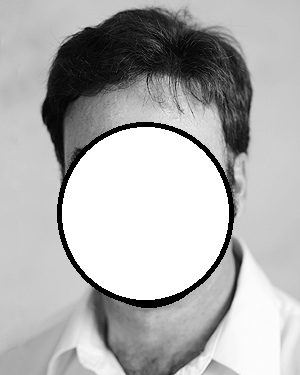
\includegraphics[width=1in,height=1.25in,clip,keepaspectratio]{author1.png}}]{First A. Author} (M'76--SM'81--F'87) and all authors may include 
biographies. Biographies are often not included in conference-related
papers. This author became a Member (M) of IEEE in 1976, a Senior
Member (SM) in 1981, and a Fellow (F) in 1987. The first paragraph may
contain a place and/or date of birth (list place, then date). Next,
the author's educational background is listed. The degrees should be
listed with type of degree in what field, which institution, city,
state, and country, and year the degree was earned. The author's major
field of study should be lower-cased. 

The second paragraph uses the pronoun of the person (he or she) and not the 
author's last name. It lists military and work experience, including summer 
and fellowship jobs. Job titles are capitalized. The current job must have a 
location; previous positions may be listed 
without one. Information concerning previous publications may be included. 
Try not to list more than three books or published articles. The format for 
listing publishers of a book within the biography is: title of book 
(publisher name, year) similar to a reference. Current and previous research 
interests end the paragraph. The third paragraph begins with the author's 
title and last name (e.g., Dr.\ Smith, Prof.\ Jones, Mr.\ Kajor, Ms.\ Hunter). 
List any memberships in professional societies other than the IEEE. Finally, 
list any awards and work for IEEE committees and publications. If a 
photograph is provided, it should be of good quality, and 
professional-looking. Following are two examples of an author's biography.
\end{IEEEbiography}

\begin{IEEEbiography}[{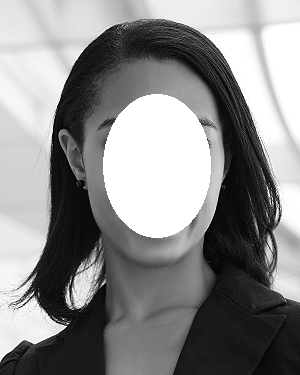
\includegraphics[width=1in,height=1.25in,clip,keepaspectratio]{author2.png}}]{Second B. Author} was born in Greenwich Village, New York, NY, USA in 
1977. He received the B.S. and M.S. degrees in aerospace engineering from 
the University of Virginia, Charlottesville, in 2001 and the Ph.D. degree in 
mechanical engineering from Drexel University, Philadelphia, PA, in 2008.

From 2001 to 2004, he was a Research Assistant with the Princeton Plasma 
Physics Laboratory. Since 2009, he has been an Assistant Professor with the 
Mechanical Engineering Department, Texas A{\&}M University, College Station. 
He is the author of three books, more than 150 articles, and more than 70 
inventions. His research interests include high-pressure and high-density 
nonthermal plasma discharge processes and applications, microscale plasma 
discharges, discharges in liquids, spectroscopic diagnostics, plasma 
propulsion, and innovation plasma applications. He is an Associate Editor of 
the journal \emph{Earth, Moon, Planets}, and holds two patents. 

Dr. Author was a recipient of the International Association of Geomagnetism 
and Aeronomy Young Scientist Award for Excellence in 2008, and the IEEE 
Electromagnetic Compatibility Society Best Symposium Paper Award in 2011. 
\end{IEEEbiography}

\begin{IEEEbiography}[{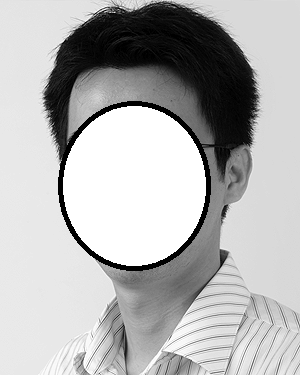
\includegraphics[width=1in,height=1.25in,clip,keepaspectratio]{author3.png}}]{Third C. Author, Jr.} (M'87) received the B.S. degree in mechanical 
engineering from National Chung Cheng University, Chiayi, Taiwan, in 2004 
and the M.S. degree in mechanical engineering from National Tsing Hua 
University, Hsinchu, Taiwan, in 2006. He is currently pursuing the Ph.D. 
degree in mechanical engineering at Texas A{\&}M University, College 
Station, TX, USA.

From 2008 to 2009, he was a Research Assistant with the Institute of 
Physics, Academia Sinica, Tapei, Taiwan. His research interest includes the 
development of surface processing and biological/medical treatment 
techniques using nonthermal atmospheric pressure plasmas, fundamental study 
of plasma sources, and fabrication of micro- or nanostructured surfaces. 

Mr. Author's awards and honors include the Frew Fellowship (Australian 
Academy of Science), the I. I. Rabi Prize (APS), the European Frequency and 
Time Forum Award, the Carl Zeiss Research Award, the William F. Meggers 
Award and the Adolph Lomb Medal (OSA).
\end{IEEEbiography}

\end{document}
